% This must be in the first 5 lines to tell arXiv to use pdfLaTeX, which is strongly recommended.
\pdfoutput=1
% In particular, the hyperref package requires pdfLaTeX in order to break URLs across lines.

\documentclass[11pt]{article}

% Change "review" to "final" to generate the final (sometimes called camera-ready) version.
% Change to "preprint" to generate a non-anonymous version with page numbers.
% \usepackage[preprint]{acl}
\usepackage[final]{acl}

% Standard package includes
\usepackage{times}
\usepackage{latexsym}
\usepackage{xcolor}
\usepackage{tcolorbox}

\usepackage{tabularx}
\usepackage{booktabs}
\usepackage{enumitem}
% For proper rendering and hyphenation of words containing Latin characters (including in bib files)
\usepackage[T1]{fontenc}
% For Vietnamese characters
% \usepackage[T5]{fontenc}
% See https://www.latex-project.org/help/documentation/encguide.pdf for other character sets

% This assumes your files are encoded as UTF8
\usepackage[utf8]{inputenc}

% This is not strictly necessary, and may be commented out,
% but it will improve the layout of the manuscript,
% and will typically save some space.
\usepackage{microtype}
\usepackage{amsmath}
\usepackage{amssymb}
\usepackage{colortbl}
\usepackage{booktabs}
\usepackage{pifont}
\usepackage{xcolor}
\usepackage{multirow}
% This is also not strictly necessary, and may be commented out.
% However, it will improve the aesthetics of text in
% the typewriter font.
\usepackage{inconsolata}

%Including images in your LaTeX document requires adding
%additional package(s)
\usepackage{graphicx}
\definecolor{darkgreen}{rgb}{0.0, 0.5, 0.0}
\newcommand{\greencheck}{\textcolor{darkgreen}{\ding{51}}}

\hypersetup{
    colorlinks=true,
    linkcolor=red,
    citecolor=cyan,
    filecolor=magenta,      
    urlcolor=cyan,
    }
% If the title and author information does not fit in the area allocated, uncomment the following
%
%\setlength\titlebox{<dim>}
%
% and set <dim> to something 5cm or larger.

\title{
% MedCoT: Medical Chain of Thought via Hierarchical Expert Authentication
MedCoT: Medical Chain of Thought via Hierarchical Expert 
}

% Author information can be set in various styles:
% For several authors from the same institution:
% \author{Author 1 \and ... \and Author n \\
%         Address line \\ ... \\ Address line}
% if the names do not fit well on one line use
%         Author 1 \\ {\bf Author 2} \\ ... \\ {\bf Author n} \\
% For authors from different institutions:
% \author{Author 1 \\ Address line \\  ... \\ Address line
%         \And  ... \And
%         Author n \\ Address line \\ ... \\ Address line}
% To start a separate ``row'' of authors use \AND, as in
% \author{Author 1 \\ Address line \\  ... \\ Address line
%         \AND
%         Author 2 \\ Address line \\ ... \\ Address line \And
%         Author 3 \\ Address line \\ ... \\ Address line}

% \author{First Author \\
%   Affiliation / Address line 1 \\
%   Affiliation / Address line 2 \\
%   Affiliation / Address line 3 \\
%   \texttt{email@domain} \\\And
%   Second Author \\
%   Affiliation / Address line 1 \\
%   Affiliation / Address line 2 \\
%   Affiliation / Address line 3 \\
%   \texttt{email@domain} \\}

\author{
 \textbf{Jiaxiang Liu\textsuperscript{1}}\ \ \
 \textbf{Yuan Wang\textsuperscript{1}}\ \ \
 \textbf{Jiawei Du\textsuperscript{2, 3}}\ \ \
 \textbf{Joey Tianyi Zhou\textsuperscript{2, 3}}\ \ \
 \textbf{Zuozhu Liu\textsuperscript{*, 1}}
\\
\\
 \textsuperscript{1} \small ZJU-Angelalign R\&D Center for Intelligence Healthcare, Zhejiang University, China\\
 % \textsuperscript{2}National University of Singapore,
 \textsuperscript{2} \small Centre for Frontier AI Research (CFAR), Agency for Science, Technology and Research (A*STAR), Singapore
\\
 \textsuperscript{3} \small Institute of High Performance Computing (IHPC), Agency for Science, Technology and Research (A*STAR), Singapore
\\
 % \small
 { \small
   % \textbf{Correspondence:} 
   % \href{mailto:zuozhuliu@intl.zju.edu.cn}
   {\tt \{jiaxiang.21, zuozhuliu\}@intl.zju.edu.cn}
 }
}

\begin{document}

\maketitle

\begin{abstract}
Artificial intelligence has advanced in Medical Visual Question Answering (Med-VQA), but prevalent research tends to focus on the accuracy of the answers, often overlooking the reasoning paths and interpretability, which are crucial in clinical settings. Besides, current Med-VQA algorithms, typically reliant on singular models, lack the robustness needed for real-world medical diagnostics which usually require collaborative expert evaluation.
To address these shortcomings, this paper presents MedCoT, a novel hierarchical expert verification reasoning chain method designed to enhance interpretability and accuracy in biomedical imaging inquiries. MedCoT is predicated on two principles: \textit{The necessity for explicit reasoning paths in Med-VQA} and \textit{the requirement for multi-expert review to formulate accurate conclusions}. The methodology involves an Initial Specialist proposing diagnostic rationales, followed by a Follow-up Specialist who validates these rationales, and finally, a consensus is reached through a vote among a sparse Mixture of Experts within the locally deployed Diagnostic Specialist, which then provides the definitive diagnosis.
Experimental evaluations on four standard Med-VQA datasets demonstrate that MedCoT surpasses existing state-of-the-art approaches, providing significant improvements in performance and interpretability. 
Code is released at \url{https://github.com/JXLiu-AI/MedCoT}.
\let\thefootnote\relax\footnotetext{* Corresponding author.}
\end{abstract}

\section{Introduction}


\begin{figure}[t!]
\centering
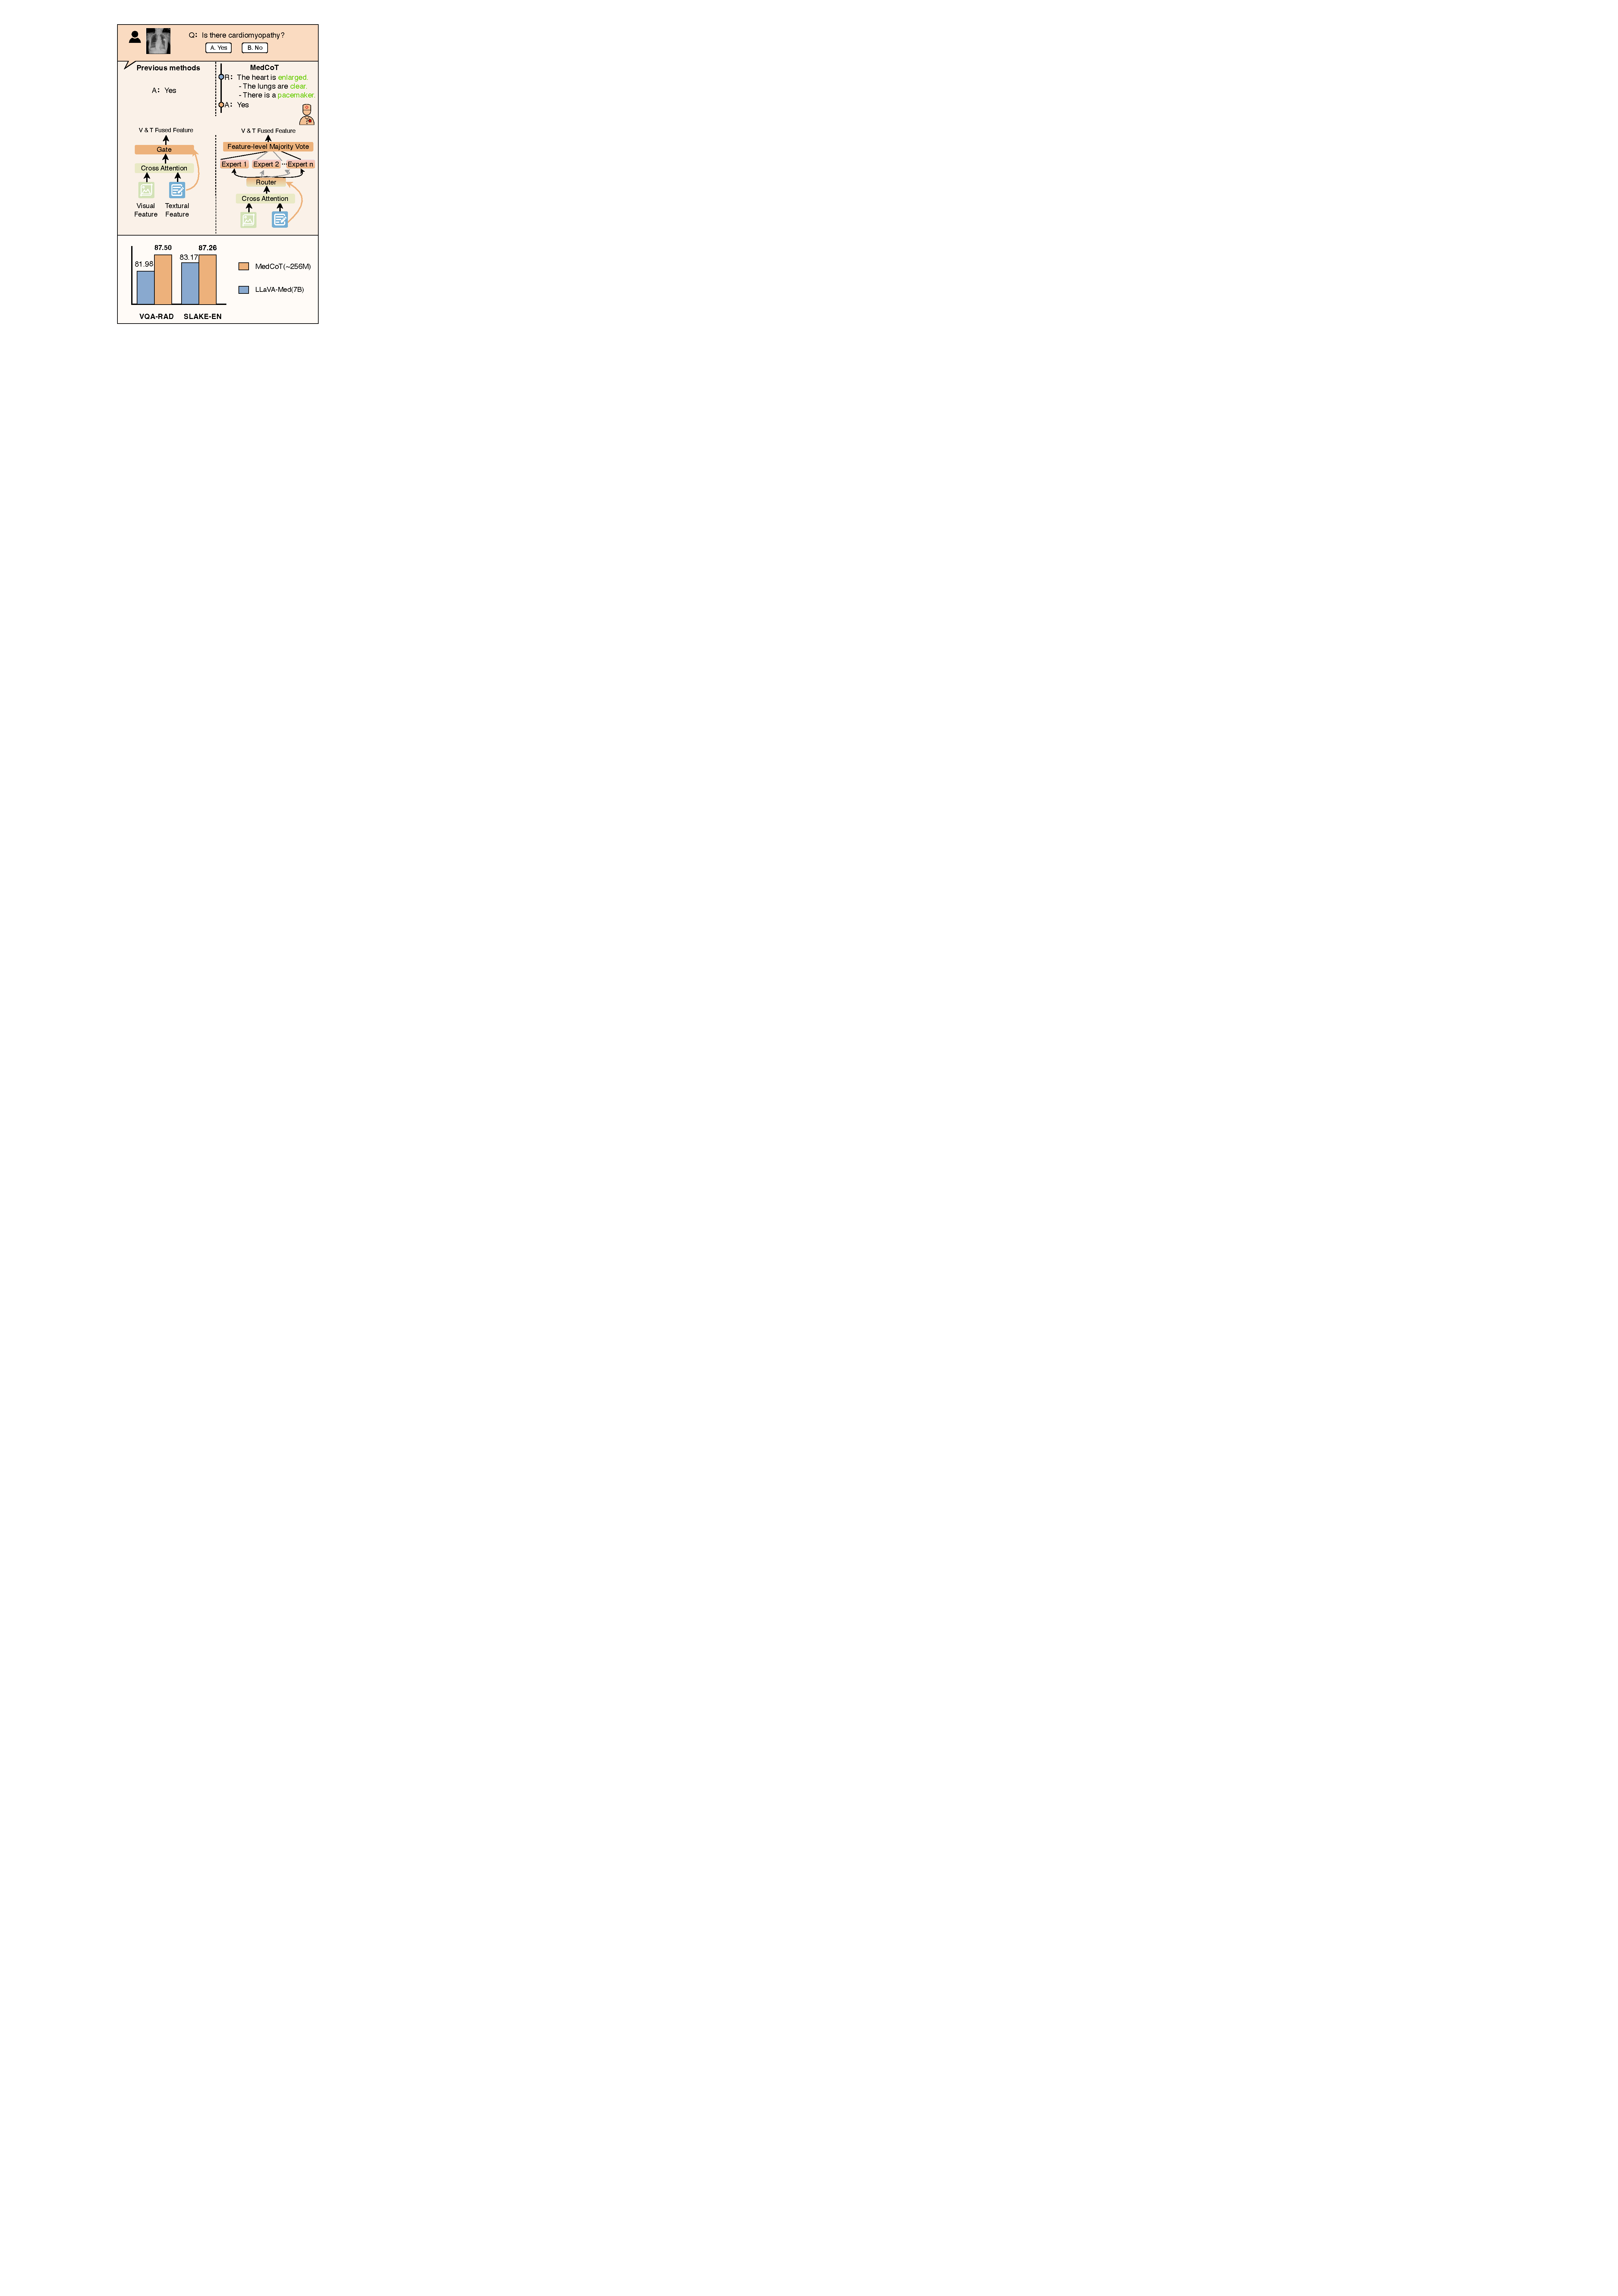
\includegraphics[width=0.45\textwidth]{image/Figure_1_v7.pdf}
\caption{
The upper figure shows a comparison of the outputs from the previous Med-VQA method and MedCoT, as well as the previous techniques in MMCoT \cite{zhang2023multimodal} versus Sparse MoE in MedCoT.
The lower figure demonstrates that MedCoT, with a model size of ~256M parameters, outperforms the 7B parameter LLaVA-Med by 5.52\% and 4.09\% (Accuracy) on the VQA-RAD and SLAKE-EN datasets. 
%The chart compares their accuracy rates.
% Comparison of (a) full fine-tuning and (b) adapter training for Med-VQA. By updating only a tiny set of adapter parameters, we can achieve better performance to full fine-tuning. $ACC$ denotes the accuracy on VQA-Rad.
} 
\label{fig1}
% \vspace{-1em}
\end{figure}

Medical Visual Question Answering (Med-VQA) has recently gained significant attention \cite{chen2022align, gong2021cross, ren2020cgmvqa, khare2021mmbert}. As a new exploration in the medical domain, Med-VQA aims to answer medical questions in natural language based on input medical images. An effective Med-VQA system can assist clinicians in interpreting medical images, thereby ensuring and accelerating the diagnostic process. For patients, automated Med-VQA services can greatly satisfy the demand for personalized health consultations \cite{liu2023parameter}.



In the field of Med-VQA, numerous attempts have been made using deep learning technologies \cite{tiong2022plug, banerjee2020weaqa, changpinyo2022all, liu2023chatgpt, gai2024medthink}.
% For instance, \citet{kim2018bilinear} introduced the Bilinear Attention Networks (BAN), an effective multimodal feature fusion technique for integrating features from visual and semantic channels, which achieved encouraging results in general VQA tasks. Inspired by the success in general VQA settings, recent studies have further explored domain-specific Med-VQA tasks. 
For instance, \citet{nguyen2019overcoming} utilized Bilinear Attention Networks (BAN) \cite{kim2018bilinear} and enhanced them for Med-VQA by incorporating a Mixed Enhanced Visual Feature (MEVF) setup consisting of pre-trained meta-learning modules and Convolutional Denoising Autoencoders (CDAE). Building on this, \citet{zhan2020medical} designed a conditional reasoning framework to boost the inference capabilities of Med-VQA models. However, these approaches often underperform in many practical scenarios, primarily due to poor capabilities in extracting and integrating features from a limited number of medical images and text data \cite{eslami2021does, song2022clip, wang2022clip}.
\citet{eslami2021does} introduced the CLIP architecture into the framework by deploying it as the visual encoder within MEVF \cite{nguyen2019overcoming}, pre-trained on the multimodal medical dataset ROCO \cite{pelka2018radiology}. Their experiments demonstrated significant improvements with the CLIP. \citet{liu2023parameter} developed VQA-Adapter, which uses a lightweight adapter and label smoothing to efficiently fine-tune the CLIP model for Med-VQA, thus reducing computational costs and mitigating overfitting.
\citet{li2024llava} proposed LLaVA-Med, which utilizes GPT-4 and a novel curriculum learning approach to efficiently train LLaVA on biomedical images, significantly enhancing Med-VQA capabilities.

However, previous Med-VQA approaches typically focused on the accuracy of the answers \cite{nguyen2019overcoming,liu2023parameter,zhan2020medical}
, where most MedVQA responses consist of a simplistic answer lacking detailed explanations or rationale, unlike in real-world scenarios where doctors not only provide answers but also explain their reasoning, professional considerations, and potential contradictions to derive a more comprehensive diagnostic insight. 
Besides, real-world diagnostics often rely on the combined experience of multiple doctors, as a single doctor's diagnosis may be biased by personal experience and may not be sufficiently accurate.
In the multimodal Chain of Thought (CoT), answering VQA questions involves providing an answer as well as a corresponding reasoning path (rationale). 
The generation of this rationale helps to improve the accuracy of the language model.
Inspired by real-world practices and multimodal CoT \citet{zhang2023multimodal,zheng2023ddcot}, integrating this paradigm into Med-VQA can enhance both the accuracy and interpretability of responses. However, implementing it faces several challenges: (1) Previous CoT methods required manual annotation of fundamental rationales, which is time-consuming, costly, and challenging to ensure consistency and completeness \cite{zhang2023multimodal,zheng2023ddcot}. (2) Reliance on a single expert model can lead to misleading conclusions. (3) Multimodal CoT has limited depth in understanding the intents of images and texts, which can restrict its effectiveness in medical contexts \cite{zhang2023multimodal}.

To address the aforementioned issues, we introduce MedCoT, a hierarchical expert-verified model for Med-VQA. Firstly, the Initial Specialist proposes preliminary diagnostic rationale based on the medical visual and text query. The Follow-up Specialist then reviews these rationales, categorizing them as valid or invalid; valid rationales are retained, while invalid ones are reassessed. 
% Finally, a locally implemented sparse mixture of experts model, functioning as a multimodal language model, casts votes to deliver the definitive diagnosis. 
% Finally, The locally implemented Diagnostic specialist consisting of sparse mixture of experts model, functioning as a multimodal language model, casts votes to deliver the definitive diagnosis. 
Finally, the locally implemented Diagnostic Specialist, consisting of a sparse Mixture of Experts (MoE) model functioning as a multimodal language model, casts votes to deliver the definitive diagnosis.
Leveraging a hierarchy of expertise, MedCoT consistently outperforms state-of-the-art (SoTA) Med-VQA methods across four extensive datasets, demonstrating impressive generalizability and interpretability, as shown in \autoref{fig1}.
Our study makes three significant contributions:

\begin{itemize}
    \item We have conducted an in-depth analysis of the challenges and insights associated with generating rationales in multimodal CoT. Our findings highlight that single specialist often fails to provide clear verifications and are more prone to errors when addressing questions about specific organs.
    \item Inspired by real-world diagnostics, we developed the hierarchical expert-verified MedCoT, which does not require manually annotated rationales. This involves three tiers of expert verification: initial, follow-up, and diagnosis. MedCoT not only provides more accurate answers but also offers refined rationales.
    \item In the diagnosis stage, we designed a sparse MoE that includes majority voting. This framework's multiple specialized experts efficiently and accurately interpret the intents of medical images and texts, enabling the Diagnostic Specialist to provide precise responses.
    
    %为了更加理解医学影像和文本的意图,我们设计了 a sparse MoE 包括了 a majority voting. 其中的多个小专家efficiently and accurately interprets the intents of medical images and texts, providing precise responses.
    
    % \item Experimental results demonstrate that MedCoT achieves state-of-the-art performance across multiple medical VQA benchmarks. It surpasses the performance of the 7-billion parameter LLaVA-Med model by 3\% on the RAD and 1.5\% on the Slake dataset, showcasing its superior accuracy and generalizability.
\end{itemize}

\vspace{1em}



% Initial Specialist \\
% Follow-up Specialist \\
% Diagnostic Specialist \\
% These instructions are for authors submitting papers to *ACL conferences using \LaTeX. They are not self-contained. All authors must follow the general instructions for *ACL proceedings,\footnote{\url{http://acl-org.github.io/ACLPUB/formatting.html}} and this document contains additional instructions for the \LaTeX{} style files.

% The templates include the \LaTeX{} source of this document (\texttt{acl\_latex.tex}),
% the \LaTeX{} style file used to format it (\texttt{acl.sty}),
% an ACL bibliography style (\texttt{acl\_natbib.bst}),
% an example bibliography (\texttt{custom.bib}),
% and the bibliography for the ACL Anthology (\texttt{anthology.bib}).

\begin{figure*}
\centering
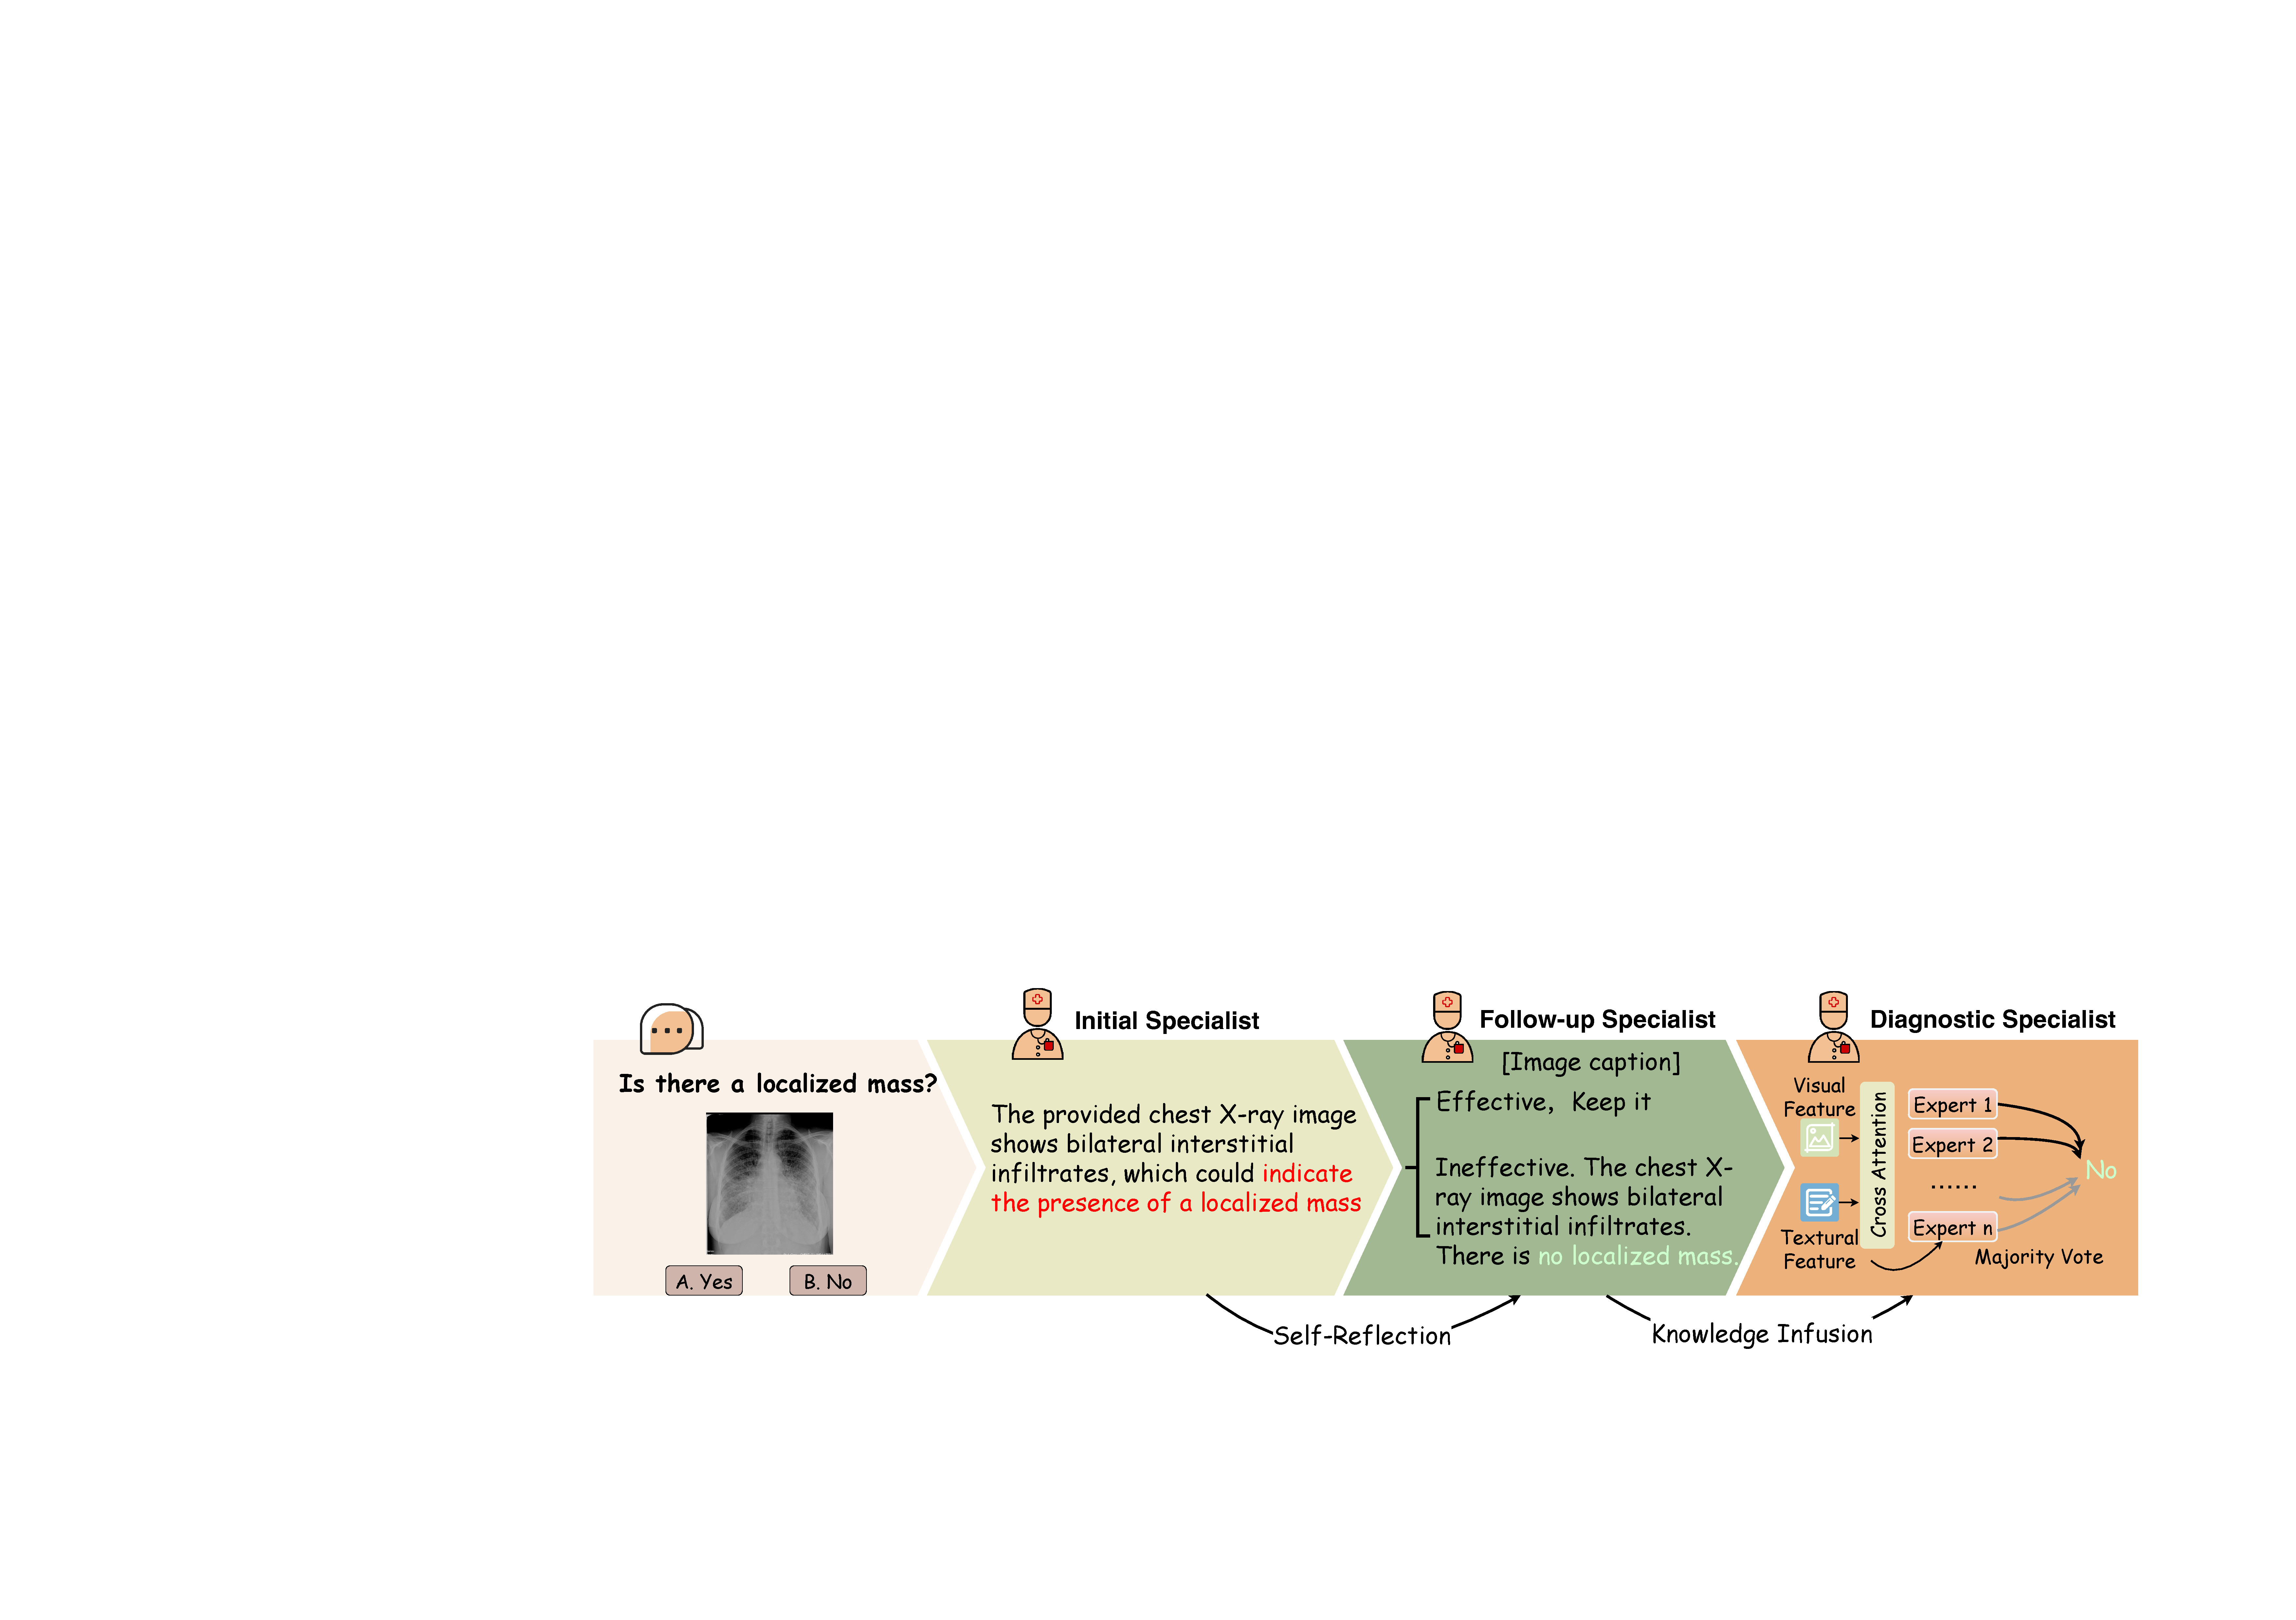
\includegraphics[width=\textwidth]{image/Figure_pipeline_v7.pdf}
\caption{
The MedCoT pipeline begins with an Initial Specialist receiving a medical question and image to generate a preliminary rationale. This rationale may have flaws (indicated in red), which are then reviewed by the Follow-up Specialist. If the rationale is deemed effective, it is retained; otherwise, it is reconsidered and a new rationale (indicated in green) is generated, along with an image caption. These elements are then integrated into the Diagnostic Specialist. Informed by all contexts, the Diagnostic Specialist, a multimodal language model with a designed sparse MoE structure, delivers the final diagnostic outcome (answer).
} 
\label{MedCoT pipeline}
\vspace{-1em}
\end{figure*}

\section{Related Work}
\vspace{-0.5em}
\subsection{Med-VQA}
VQA is a multimodal task in computer vision and natural language processing, aimed at responding to queries about images in natural language \cite{ben2019vqa,he2020pathvqa,ren2020cgmvqa}. It involves feature extraction, fusion, and inference to comprehend multimodal intents and manage feature processing. Med-VQA extends VQA into the medical domain, where robust medical knowledge is crucial for answering domain-specific questions \cite{liu2023parameter}, thus complicating feature extraction. Innovations such as Nguyen et al.'s MEVF leverage unsupervised CDAE and meta-learning to initialize weights specifically for Med-VQA \cite{nguyen2019overcoming}. Zhan et al. built upon this by developing a conditional reasoning framework to handle different types of questions \cite{zhan2020medical}, while Eslami et al. successfully implemented the CLIP model as a visual encoder, proving its effectiveness in this context \cite{eslami-etal-2023-pubmedclip}. LLaVA-Med utilizes GPT-4 and a novel curriculum learning approach for training on biomedical images \citet{li2024llava}, significantly enhancing Med-VQA capabilities. While capable of interactive dialogue, its responses do not focus on the reasoning paths leading to the answers. MedCoT differs from the aforementioned methods by not only providing precise answers but also offering reasoning paths (rationale). Moreover, its validity is confirmed through Hierarchical Expert verification, aligning more closely with real-world medical scenarios.


\subsection{Multimodal CoT}
CoT reasoning with Large Language Models (LLMs) has shown success in natural language processing. Multimodal CoT combines visual information with traditional textual CoT, integrating comprehensive data to perform reasoning tasks \cite{zhang2023multimodal,zheng2023ddcot}.
% Recent developments in zero-shot and few-shot multi-step reasoning prompts have significantly enhanced LLM reasoning capabilities \cite{zheng2023ddcot,zhang2023multimodal,zhang2024cocot}, garnering increased attention. 
Groundbreaking works in multimodal CoT  \cite{zheng2023ddcot,zhang2023multimodal,lu2022learn,lu2023chameleon,zhang2023llama} are first examined on the ScienceQA dataset. ScienceQA includes multimodal scientific questions along with annotated rationales \cite{lu2022learn}.
MM-CoT developed a two-stage framework based on ScienceQA that trains models to generate rationales from annotations, which are then used to form final answers \cite{lu2022learn}. 
With the increasing integration of open-world knowledge in LLMs, research is focusing on equipping these models with visual modalities to tackle complex visual and multimodal challenges. For instance, DDCoT \cite{zheng2023ddcot}, introduces role-specific Chains of Thought that decompose questions into subproblems and use LLMs to recombine principles, enhancing accuracy and addressing language illusions in multimodal contexts.
% Research has focused on optimizing the selection of examples based on similarity, diversity, and complexity. Other approaches have refined reasoning processes by incorporating programming methods, explicit problem decomposition, or coordination across multiple principles. 
Inspired by these advancements, we aim to adapt multimodal CoT reasoning to the medical field, aiming to improve the explainability and accuracy of Med-VQA.

\subsection{MoE}
MoE optimizes learning and prediction by combining multiple expert networks and using a gating network to determine which experts are activated based on the given input \cite{zhang2024scalable,fedus2022switch}. Sparse MoE, a variant of the MoE model, activates only a few experts during each prediction, thus efficiently utilizing computational resources and enhancing scalability \cite{shazeer2016outrageously}.
Sparse MoE models have been independently explored within the context of conditional computation in both computer vision and natural language processing domains \citet{jacobs1991adaptive,fedus2022review}. Conditional computation aims to increase the number of model parameters without proportionally increasing computational costs. This is achieved by selectively activating only the relevant parts of the model based on input-specific factors \cite{shazeer2016outrageously}. Sparse MoE models employ a learned gating mechanism that activates only a subset of experts, specifically \( k \) out of \( N \) experts, for a given input. This allows for the selection of either all experts or just a sparse mix, optimizing resource usage \citet{lepikhin2020gshard}. 
% While many studies focus on improving the gating mechanism itself, others utilize MoE models for multitasking, employing task-specific routers for each activity.


% To produce a PDF file, pdf\LaTeX{} is strongly recommended (over original \LaTeX{} plus dvips+ps2pdf or dvipdf). Xe\LaTeX{} also produces PDF files, and is especially suitable for text in non-Latin scripts.

\begin{figure}[t]
\centering

\includegraphics[width=0.5\textwidth]{image/Figure_3_v7.pdf}
\caption{Diagnostic Specialist Pipeline. After passing through a visual encoder, medical images yield visual features. Contextual textual information—including captions, rationales, and options—is processed by a text encoder to obtain textual features. These are then subjected to cross-attention for feature integration, producing combined features. These integrated features, along with textual features, are input into a Sparse MoE structure. Here, multiple specialized experts thoroughly understand the intents of both the image and text. The insights are then fed into a textual decoder, which decodes the information to produce the final answer.
%医疗图像经过视觉编码器后得到视觉特征,问题文本上下文(包括caption,rationale,选项等)经过文本编码器得到文本特征,将其进行cross attention进行特征融合得到融合特征,将融合特征与文本特征送入Sparse MoE结构,由多位专业专精的专家充分理解图像和文本的意图后,送入textual decoder,解码得到最后的answer。
} 
\label{Diagnostic}
\vspace{-1em}
\end{figure}
% \vspace{-1em}
\section{Methodology}

\subsection{Preliminaries}
Throughout this paper, we model the Med-VQA task within a multimodal CoT framework as follows: The framework takes an image \( I \) and a question \( Q \) as inputs, and outputs a reasoning rationale \( R \). This rationale \( R \) is subsequently used to generate an answer \( A \). This paradigm ensures that the process is transparent, providing a traceable path from input to conclusion, which is essential for both validating the results and improving user trust in the framework's diagnostic capabilities. We can model the Med-VQA task within a multimodal CoT as follows:
\begin{equation}
    \min_{f, g} \mathbb{E}_{(I, Q, A^*) \sim \text{Data}} \left[ L \left( g \left( f(I, Q), I, Q \right), A^* \right) \right].
\end{equation}

\( f \) is responsible for generating a rational and helpful reasoning rationale \( R \) (Initial and Follow-up Specialists), while \( g \) uses this rationale to generate the final answer \( A \) (Diagnostic Specialist). The rationale \( R \) is derived from the Initial Specialist assessments and self-reflection by the Follow-up Specialist. The final answer \( A \) is determined by a Diagnostic Specialist through a loss function \( L \), which measures the discrepancy between the predicted answer \( A \) and the true answer \( A^* \).


% \subsection{Overview}
%既关注于理解问题和图像的内容,也关注于如何利用这些理解来生成准确的答案。

\subsection{Initial Specialist}
In the initial diagnosis phase, we cue the LLMs to act as the primary rationale Diagnostic Specialist. 
We prompt the LLMs with the instruction: 
\textit{"Please proceed with a step-by-step analysis and provide a rationale"} ($prompt_{\hat{i}}$).
This is done to guide the LLMs in performing a detailed, step-by-step reasoning process. 
The textual rationale obtained from this is represented as \( R_{\hat{i}} = LLMs(T, I, prompt_{\hat{i}}) \), where \( T \) and \( I \) denote the text and image inputs, respectively. \( T \) includes textual context such as the question \( Q \) and options.
\( prompt_{\hat{i}} \) is the specific prompting strategy used to elicit the rationale. For further technical details about the prompt, please refer to the appendix.

For instance, as shown in \autoref{MedCoT pipeline}, for the question "Is there a localized mass?", we obtain a highly interpretable rationale (for the final diagnostic outcome): "The provided chest X-ray image shows bilateral interstitial infiltrates, which could indicate the presence of a localized mass".
\subsection{Follow-up Specialist}
In the follow-up diagnosis phase, we instruct LLMs to conduct self-reflection reasoning and test within the problem's context to identify effective rationales, retain them, and reconstruct ineffective ones to generate accurate rationales. Specifically, we prompt the LLMs with:
\textit{"Please judge whether this rationale is effectively valid for the question and image. If it is effective..., If the existing rationale is Ineffective..."} ($prompt_{\hat{f}}$). For the complete prompt, please refer to the appendix. We can define the Self-Reflection reasoning of the Follow-up Specialist using the following formula:
\begin{equation}
\begin{small}
R_{\hat{f}} = 
\begin{cases} 
R_{\hat{i}} & \text{if } R_{\hat{i}} = \text{Effective} \\
\text{LLMs}(T, I, {prompt}_{\hat{f}}) & \text{if } R_{\hat{i}} = \text{Ineffective},
\end{cases}
\end{small}
\end{equation}
where $R_{\hat{f}}$ is Follow-up Specialist rationale. This process helps us obtain the textual rationale needed for the diagnostic analysis, as shown in \autoref{MedCoT pipeline}.

To infuse the Diagnostic Specialist with more knowledge and bridge the gap between image and text, we utilize the Follow-up Specialist to generate image captions. This process helps to reduce the modality gap, effectively channeling this knowledge into the Diagnostic Specialist. For detailed caption prompts, please refer to the appendix.

%为了给下游的Diagnostic Specialist注入更多知识,并且弥合图像和文本的差距, we use the Follow-up Specialist to generate medical image captions to reduce the modality gap between image and text, injecting this knowledge into the Diagnostic Specialist. For detailed caption prompts, please refer to the appendix.





\subsection{Diagnostic Specialist}
We employ the designed model based on multimodal T5 combined with sparse MoE to serve as the Diagnostic Specialist, as shown in \autoref{Diagnostic}. The Diagnostic Specialist receives enriched textual context and medical imaging information to generate the final diagnostic outcome.
\subsubsection{Multimodal T5}
\autoref{Diagnostic} shows the structure of multimodal T5, including the \textit{TextualEncoder}, \textit{VisualEncoder}, \textit{Cross-Attention Network}, sparse MoE, and the \textit{TextualDecoder}. Here are the network details:

\textit{TextualEncoder} transforms natural language input \( {T} \) into the textual feature space \( F_T \in \mathbb{R}^{n \times d} \), and \textit{VisualEncoder} converts the input image \( I \) into visual features \( F_I \in \mathbb{R}^{m \times d} \). 
% This process can be formalized as \( F_{T} = \text{TextualEncoder}({T}) \) and \( F_{V} = \text{VisualEncoder}(V) \).
Here, \( n \) signifies the length of the input language text, \( d \) the dimensionality of hidden features, and \( m \) the count of image patches.
Upon obtaining the textual representation \( F_T \) and visual representation \( F_I \), our model leverages the \textit{Cross-Attention Network} for modality interaction. This network computes the attention-guided visual feature \( H_{V}^{\text{att}} \in \mathbb{R}^{n \times d} \), which selectively captures relevant visual features in response to the textual query, as delineated in the operation:
\begin{align}
        H_{V}^{\text{att}} &= \text{Softmax}\left(\frac{QK^{\top}}{\sqrt{d}}\right)V,
\end{align}
where $Q$, $K$, $V$ correspond to the query, key, and value, derived from $F_T$, $F_I$, $F_I$, respectively.

%一旦获得了H_{V}^{\text{att}} 和\( F_T \),我们利用MoE dynamically amalgamates the textual representation \( F_T \) and the attention-guided visual feature \( H_{V}^{\text{att}} \),因此有F_I = MoE (H_{V}^{\text{att}},F_T). MoE的细节如下节所示
Once the attention-guided visual feature \( H_{V}^{\text{att}} \) and the textual representation \( F_T \) are obtained, we construct the MoE to dynamically amalgamate them, resulting in \( F_F = \text{MoE} (H_{V}^{\text{att}}, F_T) \). Details of the MoE are provided in the following section.
$F_{\text{ F}}$ is input into the \textit{TextualDecoder} to generate answer
$A = \text{TextualDecoder}(F_{\text{F}})$, as shown in \autoref{Diagnostic}. 

% The \textit{Gated Dense Layer} dynamically amalgamates the textual representation \( F_T \) and the attention-guided visual feature \( H_{V}^{\text{att}} \), deriving the fusion coefficient \( \lambda \) through a sigmoid-activated linear combination of these modalities:
% \begin{align}
%          \lambda &= \text{Sigmoid}(W_lF_T + W_vH_{V}^{\text{att}}),
% \end{align}
% where $W_l$ and $W_v$ are the model parameters learned during training which optimize the blend of information from the textual and visual streams. 
% The integrated output $F_{\text{I}} \in\mathbb{R}^{n \times d}$ is then computed as a weighted sum of $F_T$ and $H_{V}^{att}$, 
% moderated by $\lambda$:
% \begin{align}
%     F_{\text{I}} &= (1-\lambda) \cdot F_{\text{T}} + \lambda \cdot H_{V}^{\text{att}}.
% \end{align}



In the training, refinements enable predicted answers (A) to more accurately approximate label answers. Specifically,The model $f$ with input maximizes the likelihood of the correct sequence $Y = {A}$. The loss function $L$, which is the negative log-likelihood over all tokens, is given by: $L = -\sum_{n=1}^{N} \log p(Y_n | X, Y_1^{n-1})$, where $N$ is the number of tokens, and $p(Y_n | X, Y_1^{n-1})$ is the probability of predicting the correct $n$-th token in $Y$. 
\subsubsection{MoE}

% \textbf{Sparse MoE}
In the multimodal CoT, a crucial step is understanding the intent of both the image and the text and responding accordingly. 
However, previous methods primarily utilized gates for integration, where the gate function \( \lambda = \text{Sigmoid}(W_l F_T + W_v H_V^{\text{att}}) \) weights the importance of the image relative to the source text, with \( W_l \) and \( W_v \) as learnable parameters (see Appendix) \cite{zhang2023multimodal, zheng2023ddcot}.
Which, according to our experiments, shows that the gate is insufficient (\autoref{ablation}).
% which, according to our experiments, gate is often insufficient. 
Therefore, MedCoT proposes constructing a MoE for the integration process.

The Sparse MoE implements a top-k sparse mixture of experts \cite{fedus2022switch}, leveraging multiple Sparse Experts to specialize in processing complex Med-VQA data. 
This module dynamically selects the top-k experts for each input based on gating scores, as shown in \autoref{Diagnostic}. 
%得到experts的输出后,我们利用Feature-level Majority Vote来aggregates their outputs

%让每位选出的专家处理擅长的数据,如Figure6展示了擅长处理Head问题的专家。
% Sparse MoE provide a robust framework for building scalable, efficient, and adaptive neural networks. Their ability to dynamically select and aggregate outputs from a pool of experts enables them to handle complex tasks more effectively.
After obtaining the outputs from the experts, we use Feature-level Majority Vote to aggregate their outputs.
The weight of each expert is calculated using the following formula:
% \[
% \begin{small}
% \text{weights}_i = \text{softmax}(\text{values})_i = \frac{e^{\text{top\_k\_values}_i}}{\sum_{j=1}^{k} e^{\text{top\_k\_values}_j}}
% \end{small}
% \]
%\[
% \begin{small}
\begin{align}
    \text{W}_i = \text{softmax}(\text{V}^{\text{top k}})_i = \frac{e^{\text{V}^{\text{top k}}_i}}{\sum_{j=1}^{k} e^{\text{V}^{\text{top k}}_j}},
\end{align}
% \end{small}
%\]

% \[\small
% \text{result}_{F_f} = \sum_{i=1}^{k} \text{weights}_i \cdot \text{indices}^{\text{top k}}_i
% \]

where \(\text{W}_i\) is the weight of the \(i\)-th selected expert, and \(\text{V}^{\text{top k}}_i\) is the score of the \(i\)-th selected expert.
For each feature \( F_f \), the final result of Feature-level Majority Vote is calculated by weighted averaging the outputs of all selected experts:
% \[
% \text{result}_{F_f} = \sum_{i=1}^{k} \text{W}_i \cdot \text{expert}^{\text{output}}_{\text{indices}^{\text{top k}}_i, F_f},
% \]
\begin{align}
    {E}_{F_f} = \sum_{i=1}^{k} \text{W}_i \cdot E_{i, F_f} ,
\end{align}
% {E}_{F_f} = \sum_{i=1}^{k} \text{W}_i \cdot E_{i, F_f} ,
% \]
where \({E}_{F_f}\) is the value of the final result for feature \( F_f \), and \(E_{i, F_f}\) is the output of the \(i\)-th selected expert for feature \( F_f \). Then,
\(\lambda = \text{Sigmoid}({E}_{F_f}) \).
Finally, this results in \( F_f \) are as follows:
\begin{align}
    F_{\text{F}} &= (1-\lambda) \cdot F_{\text{T}} + \lambda \cdot H_{V}^{\text{att}}.
\end{align}


The sparse MoE network allows each selected expert to handle data they specialize in, as demonstrated in \autoref{rad}, which shows experts proficient in addressing head-related issues.

% The first line of the file must be
% \begin{quote}
% \begin{verbatim}
% \documentclass[11pt]{article}
% \end{verbatim}
% \end{quote}

% To load the style file in the review version:
% \begin{quote}
% \begin{verbatim}
% \usepackage[review]{acl}
% \end{verbatim}
% \end{quote}
% For the final version, omit the \verb|review| option:
% \begin{quote}
% \begin{verbatim}
% \usepackage{acl}
% \end{verbatim}
% \end{quote}

% To use Times Roman, put the following in the preamble:
% \begin{quote}
% \begin{verbatim}
% \usepackage{times}
% \end{verbatim}
% \end{quote}
% (Alternatives like txfonts or newtx are also acceptable.)

% Please see the \LaTeX{} source of this document for comments on other packages that may be useful.

% Set the title and author using \verb|\title| and \verb|\author|. Within the author list, format multiple authors using \verb|\and| and \verb|\And| and \verb|\AND|; please see the \LaTeX{} source for examples.

% By default, the box containing the title and author names is set to the minimum of 5 cm. If you need more space, include the following in the preamble:
% \begin{quote}
% \begin{verbatim}
% \setlength\titlebox{<dim>}
% \end{verbatim}
% \end{quote}
% where \verb|<dim>| is replaced with a length. Do not set this length smaller than 5 cm.


\begin{figure}[t]
\centering
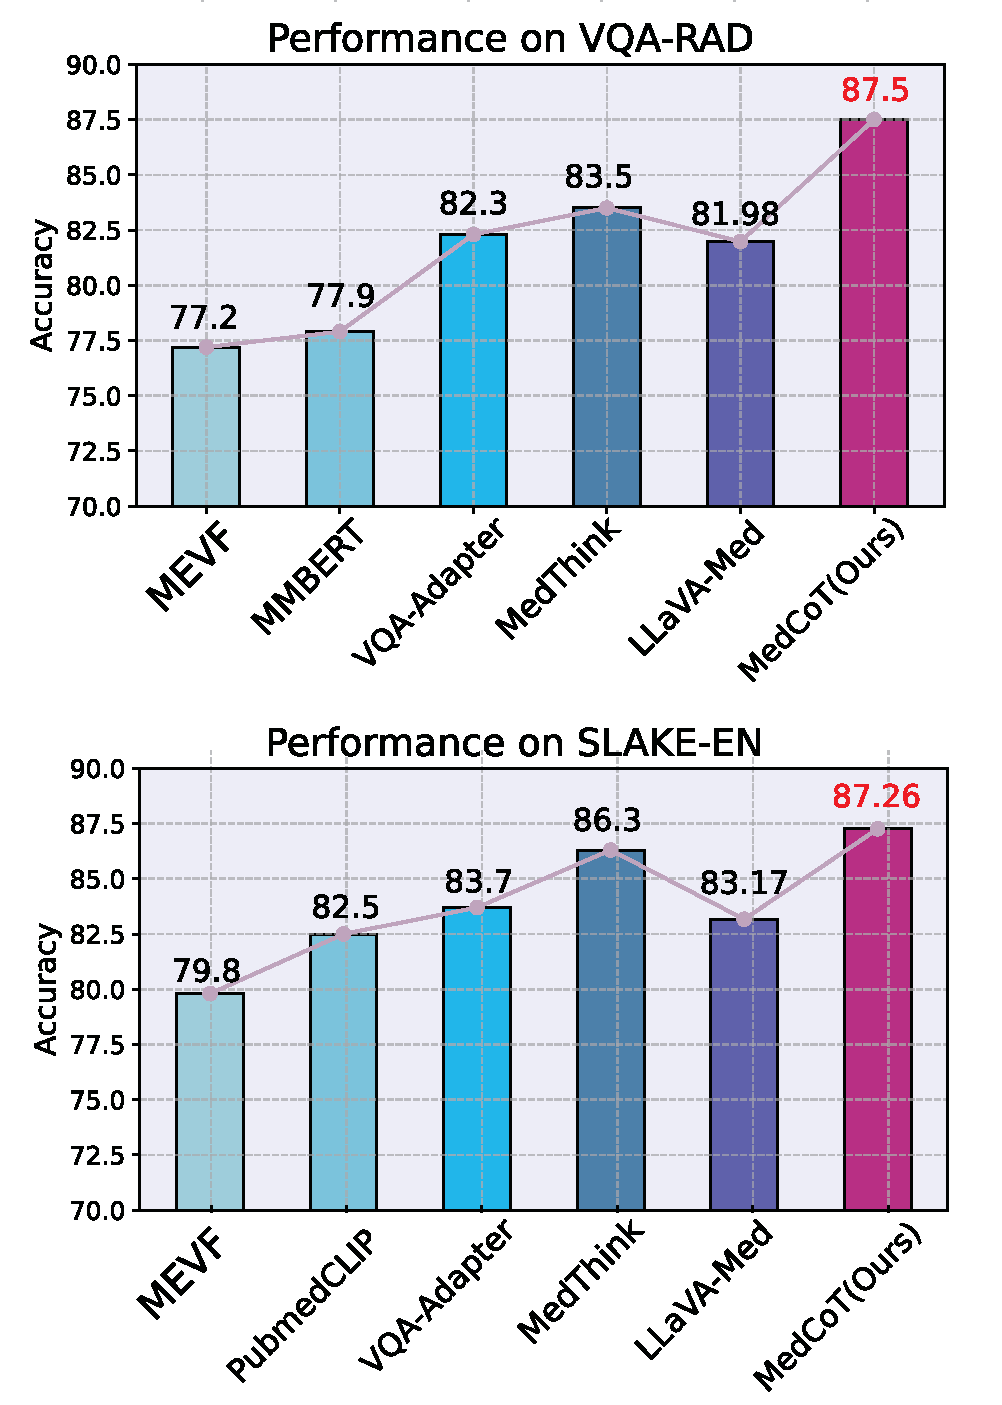
\includegraphics[width=0.4\textwidth]{image/Performance5.pdf}
\caption{
MedCoT is compared with various SoTA methods on closed questions on the VQA-RAD and SLAKE-EN datasets. MedCoT not only achieves SoTA accuracy in answers but also provides reasoning paths (rationale). The metric used is Accuracy (\%).
} 
\label{performance}
\vspace{-1em}
\end{figure}

\begin{figure*}
\centering
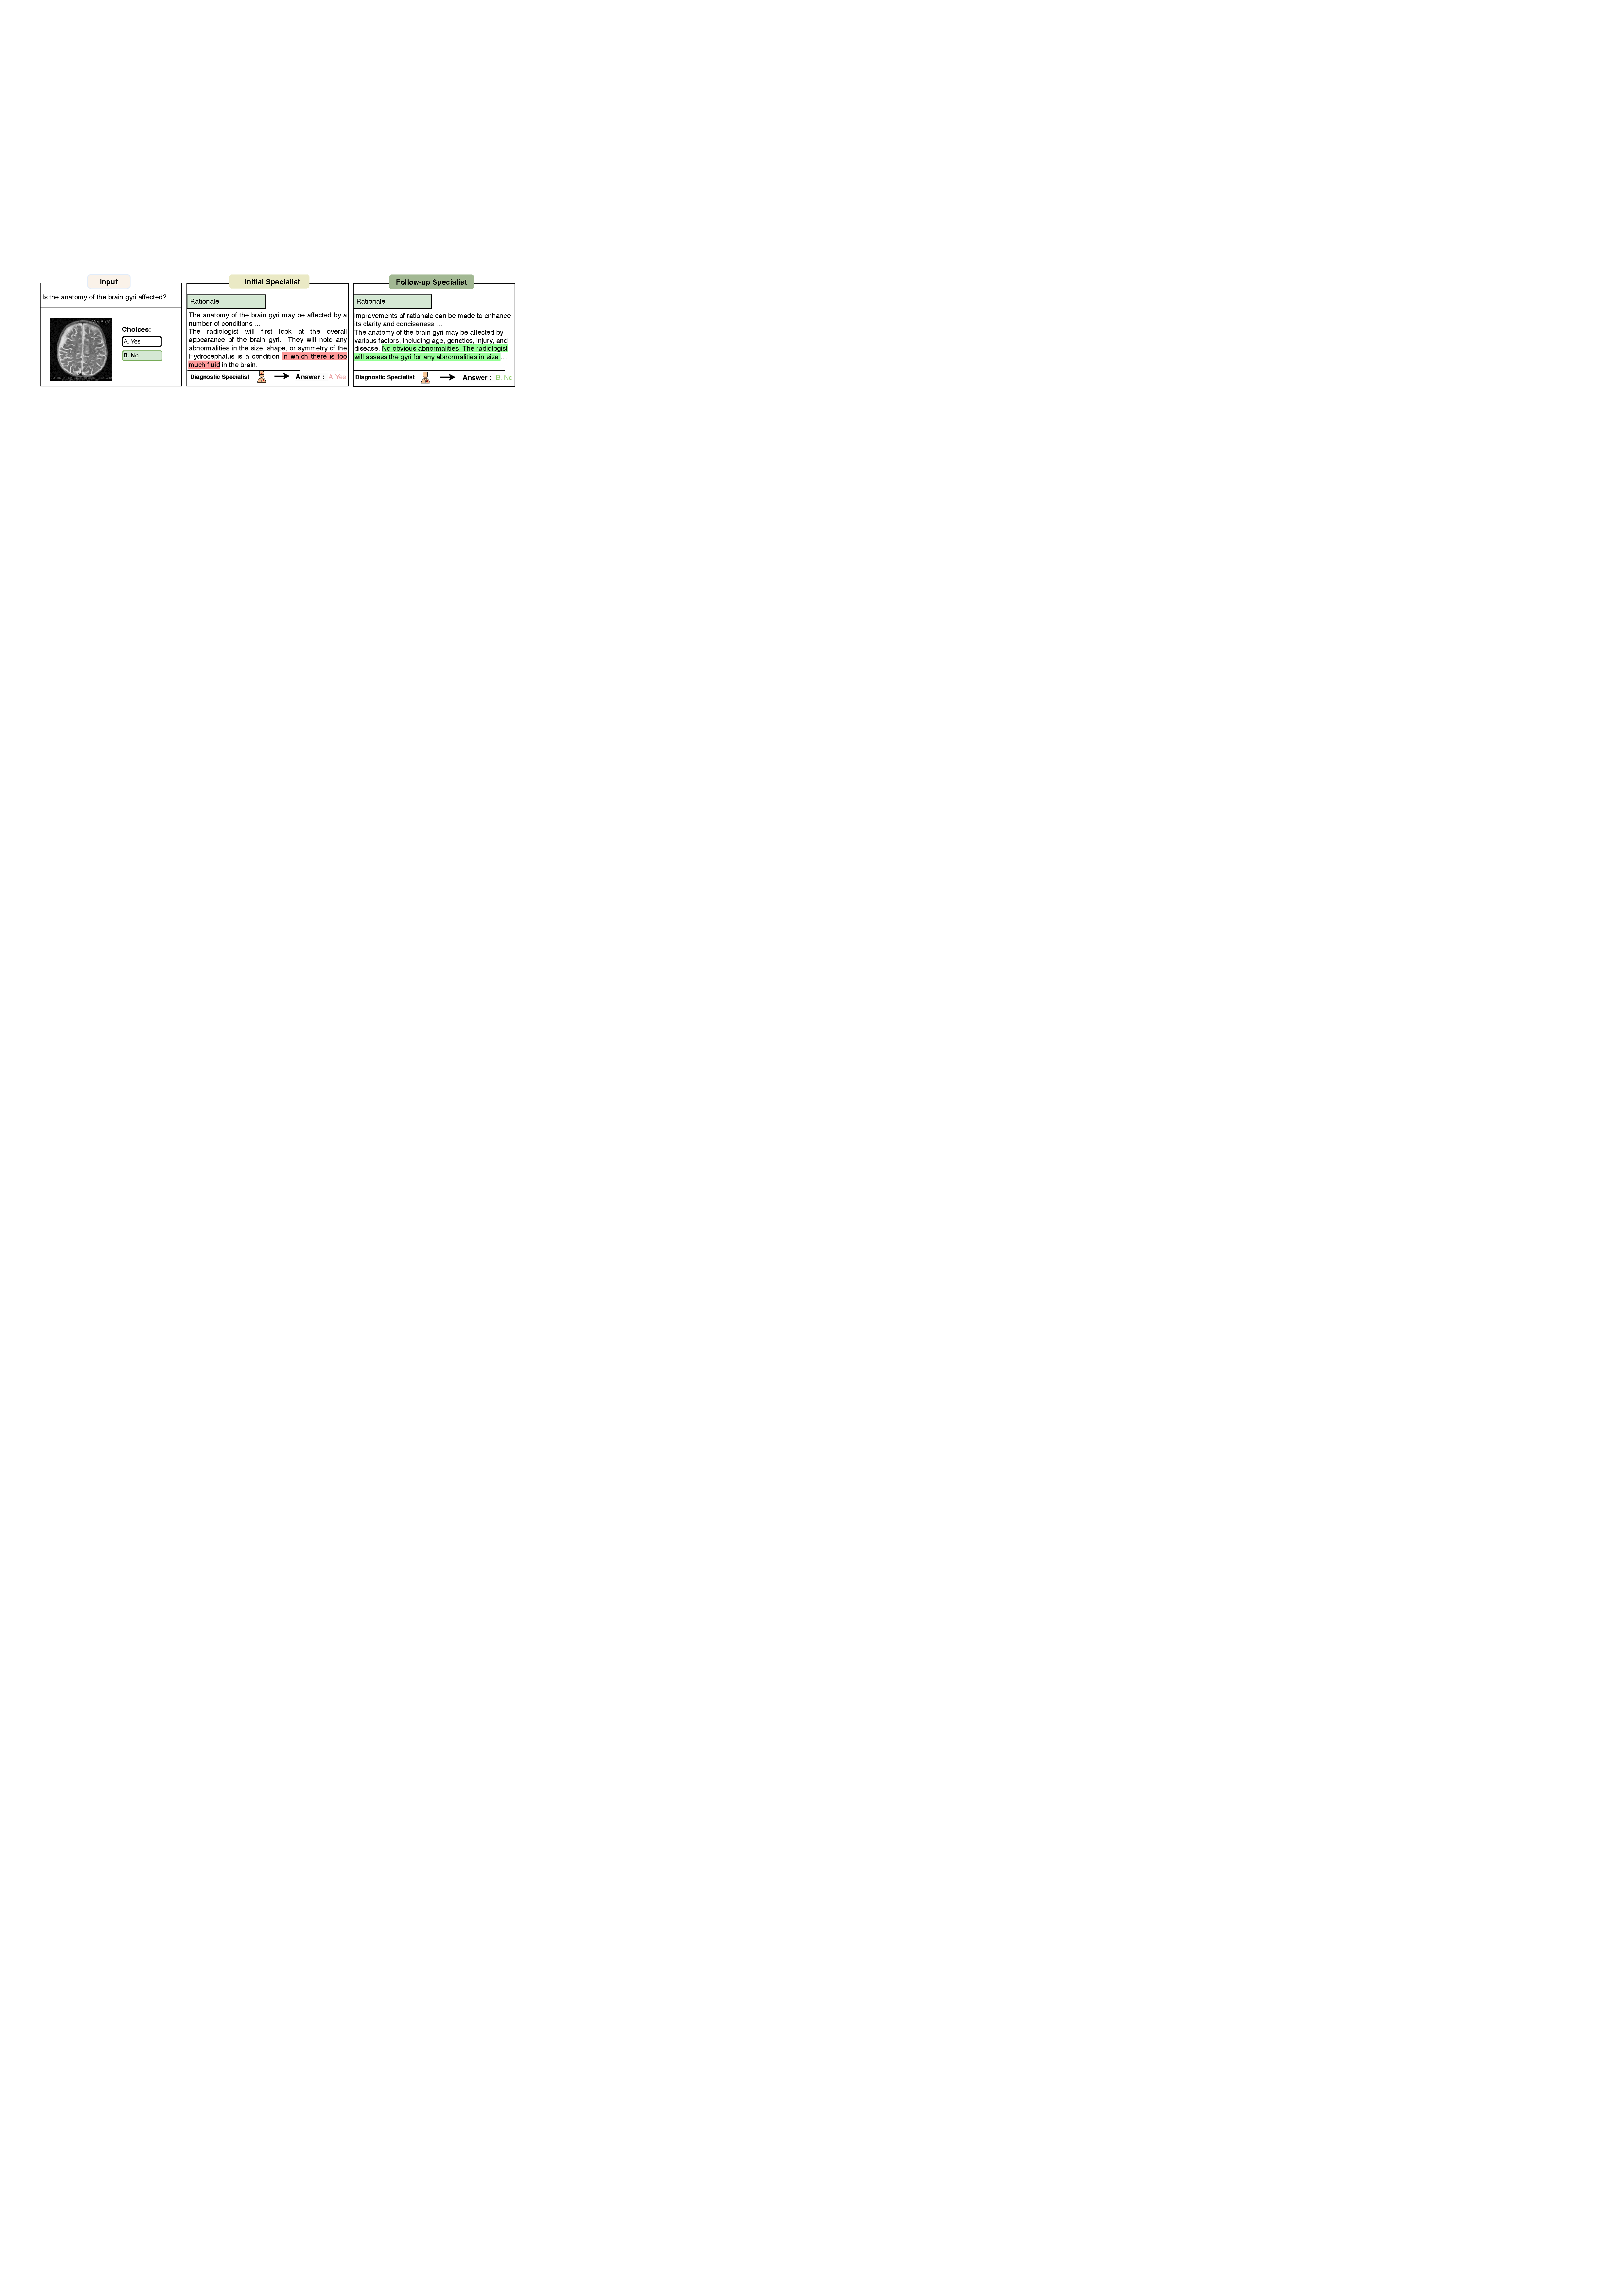
\includegraphics[width=\textwidth]{image/Figure_case1_v3.pdf}
\caption{
The MedCoT pipeline begins with an Initial Specialist receiving a medical question and image to generate a preliminary rationale. This rationale may have flaws (indicated in red), which are then reviewed by the Follow-up Specialist. If the rationale is deemed effective, it is retained; otherwise, it is reconsidered and a new rationale (indicated in green) is generated, along with an image caption. These elements are then integrated into the Diagnostic Specialist. Informed by all context, the Diagnostic Specialist, a multimodal language model with a designed sparse MoE structure, delivers the final diagnostic outcome (answer).
} 
\label{case1}
% \vspace{-1em}
\end{figure*}

\section{Experiments}

\subsection{Experimental Setting}
In MedCoT framework, the encoder and decoder from Flan-T5 \cite{khashabi2020unifiedqa,raffel2020exploring} are integrated as TextualEncoder($\cdot$) and TextualDecoder($\cdot$), respectively. Additionally, DETR \cite{carion2020end} is employed as VisualEncoder($\cdot$). 
% This integration facilitates the construction of our experimental model.
Our Diagnostic Specialist model was trained 100 epochs with a learning rate of $8e-5$ and a batch size of 8. 
To demonstrate the effects of MedCoT, four benchmark datasets are used for validation in the medical VQA domain: VQA-RAD \cite{lau2018dataset}, SLAKE-EN \cite{liu2021slake}, Med-VQA-2019 \cite{abacha2019vqa}, and PathVQA \cite{he2020pathvqa}, with detailed statistics provided in Appendix. 
All experiments were conducted using PyTorch \cite{paszke2019pytorch} and HuggingFace \cite{wolf2020transformers}, implemented on 4 NVIDIA GEFORCE RTX 3090 GPUs. Accuracy is utilized as the evaluation metric. 
For LLMs, Gemini Pro 1.5 version is used for our Initial Specialist and Follow-up Specialist. The more experimental details can be found in the Appendix.


\begin{figure}
\centering
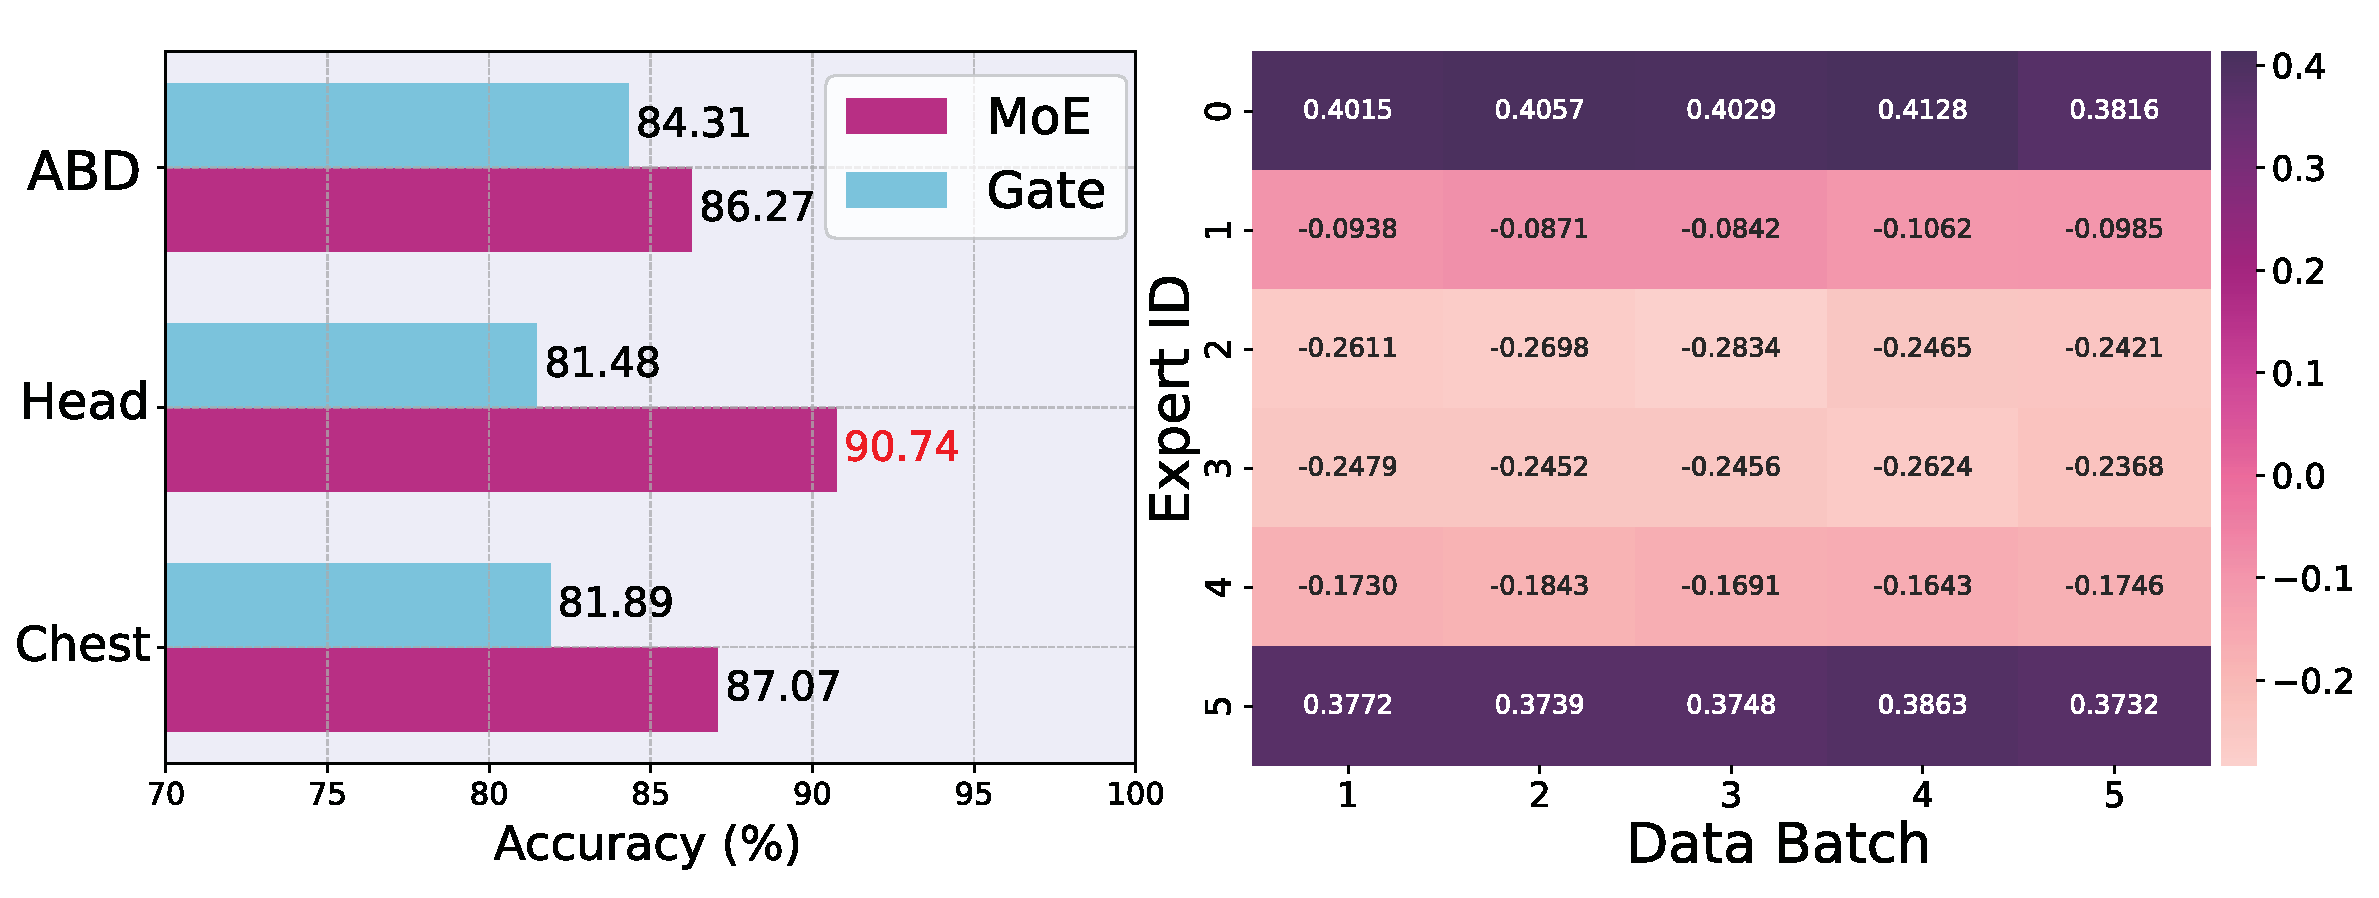
\includegraphics[width=0.5\textwidth]{image/RAD-v4.pdf}
\caption{
The Diagnostic Specialist's sparse MoE shows varying accuracy levels for different organ-related questions in VQA-RAD. 
'ABD' represents abdominal-related questions, 'Head' refers to head-related questions, and 'Chest' refers to chest-related questions.
It can be observed that head-related questions saw an improvement of nearly 10 \%. We visualized the weights of the experts (right figure). Notably, in the top 2 expert selections, the model chose Expert 0 and Expert 5 to understand the intents of the "head" image and text. 
% Experts 0 and 5 can be considered as Head specialists, proficient in diagnosing issues related to head organs.
%Diagnostic Specialist中的sparse MoE在VQA-RAD数据集上不同器官的问题的准确率的表现,ABD代表腹部器官的问题,Head代表与Head器官相关的问题,Chest代表Chest的问题。
%可以观察到,与Head器官相关的问题,提升了接近10%的百分点,我们将Expert的权重进行可视化,如下图所示,可见,在Top2的专家选择上,模型选择了Expert 0 和Expert 5来理解图像与文本的意图,可以将Expert 0和Expert视为Head专家,擅长于诊断与Head器官的问题。
} 
\label{rad}
% \vspace{-1em}
\end{figure}

\begin{figure*}
\centering
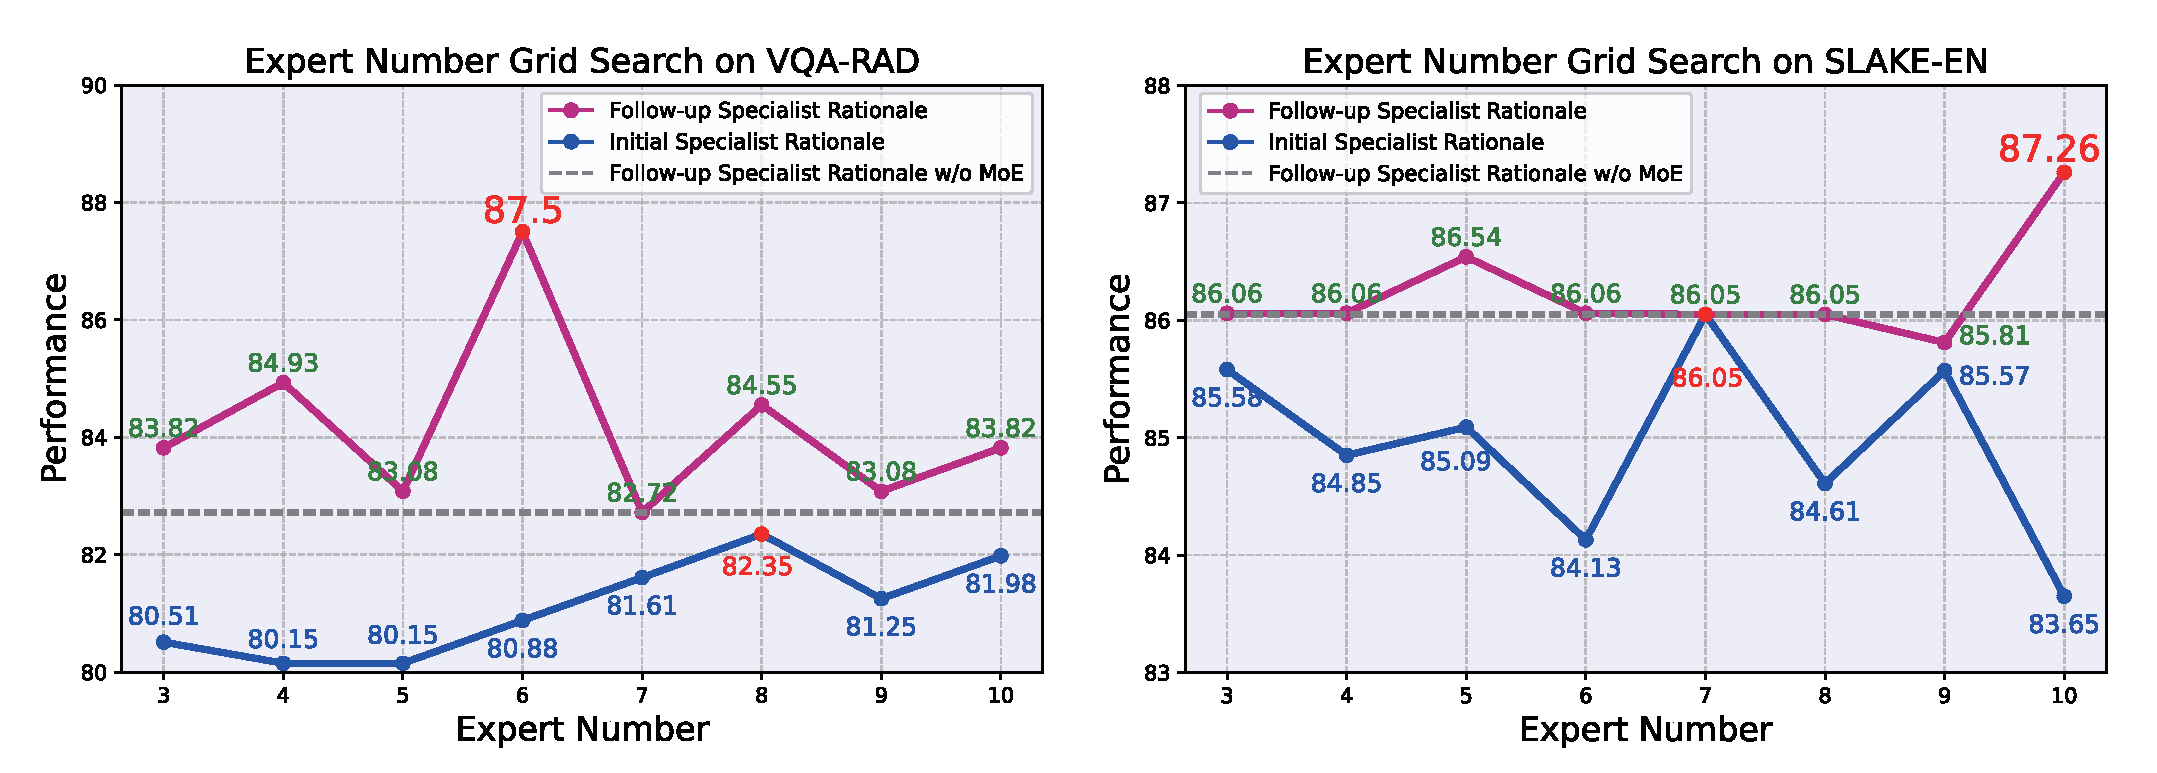
\includegraphics[width=0.9\textwidth]{image/zhexiantu_all_v6.pdf}
\caption{The expert number grid search on two datasets. The blue line represents the results from training with Initial Specialist rationales and grid search of expert numbers in the Diagnostic Specialist. The purple line represents results from using the Follow-up Specialist rationales and grid searching expert numbers. 
The gray line represents the results of the Diagnostic Specialist using Follow-up Specialist rationales, conducted without the sparse MoE.
} 
\label{zhexiantu-all}
\vspace{-1em}
\end{figure*}



\subsection{Main Results}
We evaluate the performance of MedCoT on the VQA-RAD and SLAKE-EN datasets, benchmarking them against established models like MEVF \cite{nguyen2019overcoming}, MMBERT \cite{tiong-etal-2022-plug}, PubMedCLIP \cite{eslami-etal-2023-pubmedclip}, VQA-Adapter \cite{liu2023parameter}, MedThink \cite{gai2024medthink}, LLaVA-Med \cite{li2024llava}. 

Our performance evaluation is divided into two parts, focusing separately on closed-end and open-end questions. Closed-end questions, structured as multiple-choice questions with a single correct answer, are assessed using accuracy as the performance metric, as shown in \autoref{performance}.
In facing closed-end questions, 
% the ``Explanation" method surpasses the ``Reasoning" and ``Two-Stage Reasoning" methods with accuracy of 83.5\% on the VQA-RAD dataset and 86.3\% on the SLAKE-EN dataset, marking improvements of 4.0\% and 3.8\%, respectively, over the state-of-the-art PubMedCLIP model.
%MedCoT在VQA-RAD和SLAKE-EN数据集上超越了一众SoTA方法,值得一提的是。MedCoT以223M参数的微调尺寸,在性能上超越了7B参数的LLaVA-Med方法,且分别超越了5.52%以及4.09%,并且相对于先前方法,MedCoT能够清楚的显示推理路径rationale,如Figure1所示
MedCoT surpasses a range of SoTA methods on the VQA-RAD and SLAKE-EN datasets. Notably, MedCoT achieved improvements of 27.21\% and 14.66\% over Gemini on the two datasets, demonstrating the unreliability of a single model. Besides, MedCoT, with a fine-tuning size of approximately 256M parameters, outperforms the 7B parameter LLaVA-Med (trained on extensive medical data), exceeding it by 5.52\% and 4.09\% on two datasets, respectively. Moreover, compared to previous methods, MedCoT clearly displays the reasoning paths (rationale), as illustrated in \autoref{MedCoT pipeline}.
More comparative method results can be seen in  Appendix.

In contrast, open-end questions allow for a range of answers due to their inherent nature. The answers generated by MedCoT are difficult to match precisely against the dataset. Therefore, we employ text generation metrics such as Rouge and BLEU to evaluate MedCoT's performance.
We conducted experiments on the open-end VQA-RAD and SLAKE-EN, with results shown in the Appendix. 
% The Rouge score, similar to "recall," emphasizes the completeness of the generated text, while the BLEU score, akin to "precision," highlights its accuracy. 
MedCoT demonstrated higher Rouge and BLEU scores on the VQA-RAD and SLAKE-EN dataset, surpassing MedThink \cite{gai2024medthink}.
% with Rouge-1 and BLEU-1 reaching 66.30\% and 61.29\%, respectively, surpassing MedThink \cite{gai2024medthink}. 
Besides, MedCoT also showed higher scores on the SLAKE-EN.

Additionally, we evaluated MedCoT's performance on the Med-VQA-2019 and PathVQA datasets, as shown in Appendix. The results indicate that MedCoT consistently achieves SoTA results compared to the majority of SoTA methods.

%我们在VQA-RAD以及SLKAE-EN的open-end数据集上,进行了实验,实验结果如Apeendix Table所示,Rouge得分与“召回率”类似,强调生成文本的完整性,而BLEU得分类似于“精确度”,强调生成文本的精确性。MedCoT在VQA-RAD数据集上展示了更高的Rouge和BLEU得分,其中Rouge-1、BLEU-1、分别达到了66.30%、61.29%超越了MedThink。此外,在SLAKE-EN数据集上也展示了更高的得分。

%此外,我们还在Med-VQA-2019和PathVQA的数据集上评估了MedCoT的性能,如Table 1所示,实验结果表明,MedCoT依然能够在绝大多数方法的对比下取得SoTA的结果。

%其中Rouge-2、BLEU-1、BLEU-2、BLEU-3和BLEU-4分别为23.1%、23.1%、39.5%、24.5%、15.8%和10.3%。"推理"方法在VQA-RAD和SLAKE数据集上均保持了稳健的性能;在VQA-RAD数据集上,Rouge-2、BLEU-3和BLEU-4分别达到了20.3%、14.0%和8.9%,而在SLAKE-EN数据集上,Rouge-1、Rouge-L和BLEU-1分别为53.5%、32.1%和39.5%。这些结果突显了针对不同类型开放式问题,采用多样化方法的必要性。
%此外,我们还在Med-VQA-2019和PathVQA的数据集上评估了MedCoT的性能,如Table 1所示,

% With open-end questions, different methods show distinct advantages. The Rouge scores, similar to the ``Recall", emphasizes the completeness of the generated text, while the BLEU scores, akin to the ``Precision", stresses the preciseness of the generated text. The ``Explanation" method demonstrates higher Rouge and BLEU scores on the VQA-RAD dataset, with Rouge-1, Rouge-L, BLEU-1, BLEU-2, and BLEU-3 reaching 50.2\%, 29.5\%, 38.3\%, 22.9\%, and 14.0\%, respectively. The ``Two-Stage Reasoning" method showcases higher scores on the SLAKE-EN dataset, with Rouge-2, BLEU-1, BLEU-2, BLEU-3, and BLEU-4 at 23.1\%, 23.1\%, 39.5\%, 24.5\%, 15.8\%, and 10.3\%, respectively. The ``Reasoning" method maintains robust performance across both the VQA-RAD and SLAKE datasets; on the VQA-RAD dataset, Rouge-2, BLEU-3, and BLEU-4 reached 20.3\%, 14.0\%, and 8.9\%, respectively, while on the SLAKE-EN dataset, Rouge-1, Rouge-L, and BLEU-1 are 53.5\%, 32.1\%, and 39.5\%, respectively. These outcomes highlight the necessity of diverse methods for various types of open-end questions.

% \begin{table}
% \centering
% \setlength{\extrarowheight}{0pt}
% \addtolength{\extrarowheight}{\aboverulesep}
% \addtolength{\extrarowheight}{\belowrulesep}
% \setlength{\aboverulesep}{0pt}
% \setlength{\belowrulesep}{0pt}
% \caption{Ablation Study on MedCoT}
% \resizebox{\linewidth}{!}{
% \begin{tabular}{cc|ccc} 
% \toprule
% Follow-up & MoE          & VQA-RAD                                        & SLAKE-EN                                        & Med-2019                                         \\ 
% \hline
% \greencheck         &              & 82.72                                         & 86.05                                          & 78.12                                           \\
%                      & \greencheck & 80.88                                         & 83.65                                          & 78.12                                           \\
% \greencheck         & \greencheck & {\cellcolor[rgb]{1,0.875,0.757}}\textbf{87.50} & {\cellcolor[rgb]{1,0.875,0.757}}\textbf{87.26} & {\cellcolor[rgb]{1,0.875,0.757}}\textbf{82.81}  \\
% \bottomrule
% \end{tabular}
% }
% \end{table}

\begin{table}
\centering
\small
\setlength{\extrarowheight}{0pt}
\addtolength{\extrarowheight}{\aboverulesep}
\addtolength{\extrarowheight}{\belowrulesep}
\setlength{\aboverulesep}{0pt}
\setlength{\belowrulesep}{0pt}
\caption{Ablation Study on MedCoT}
\label{xiaorong}
\begin{tabular}{cc|cc} 
\toprule
Follow-up & MoE & VQA-RAD                                        & SLAKE-EN                                        \\ 
\hline
          &     & 77.57                                          & 83.17                                           \\
   \greencheck       &     & 82.72                                          & 86.05                                           \\
          &  \greencheck   & 80.88                                          & 83.65                                           \\
  \greencheck        &  \greencheck   & {\cellcolor[rgb]{1,0.875,0.757}}\textbf{87.50} & {\cellcolor[rgb]{1,0.875,0.757}}\textbf{87.26}  \\
\bottomrule
\end{tabular}
% \vspace{-1em}
\end{table}







% \begin{figure*}
% \centering
% 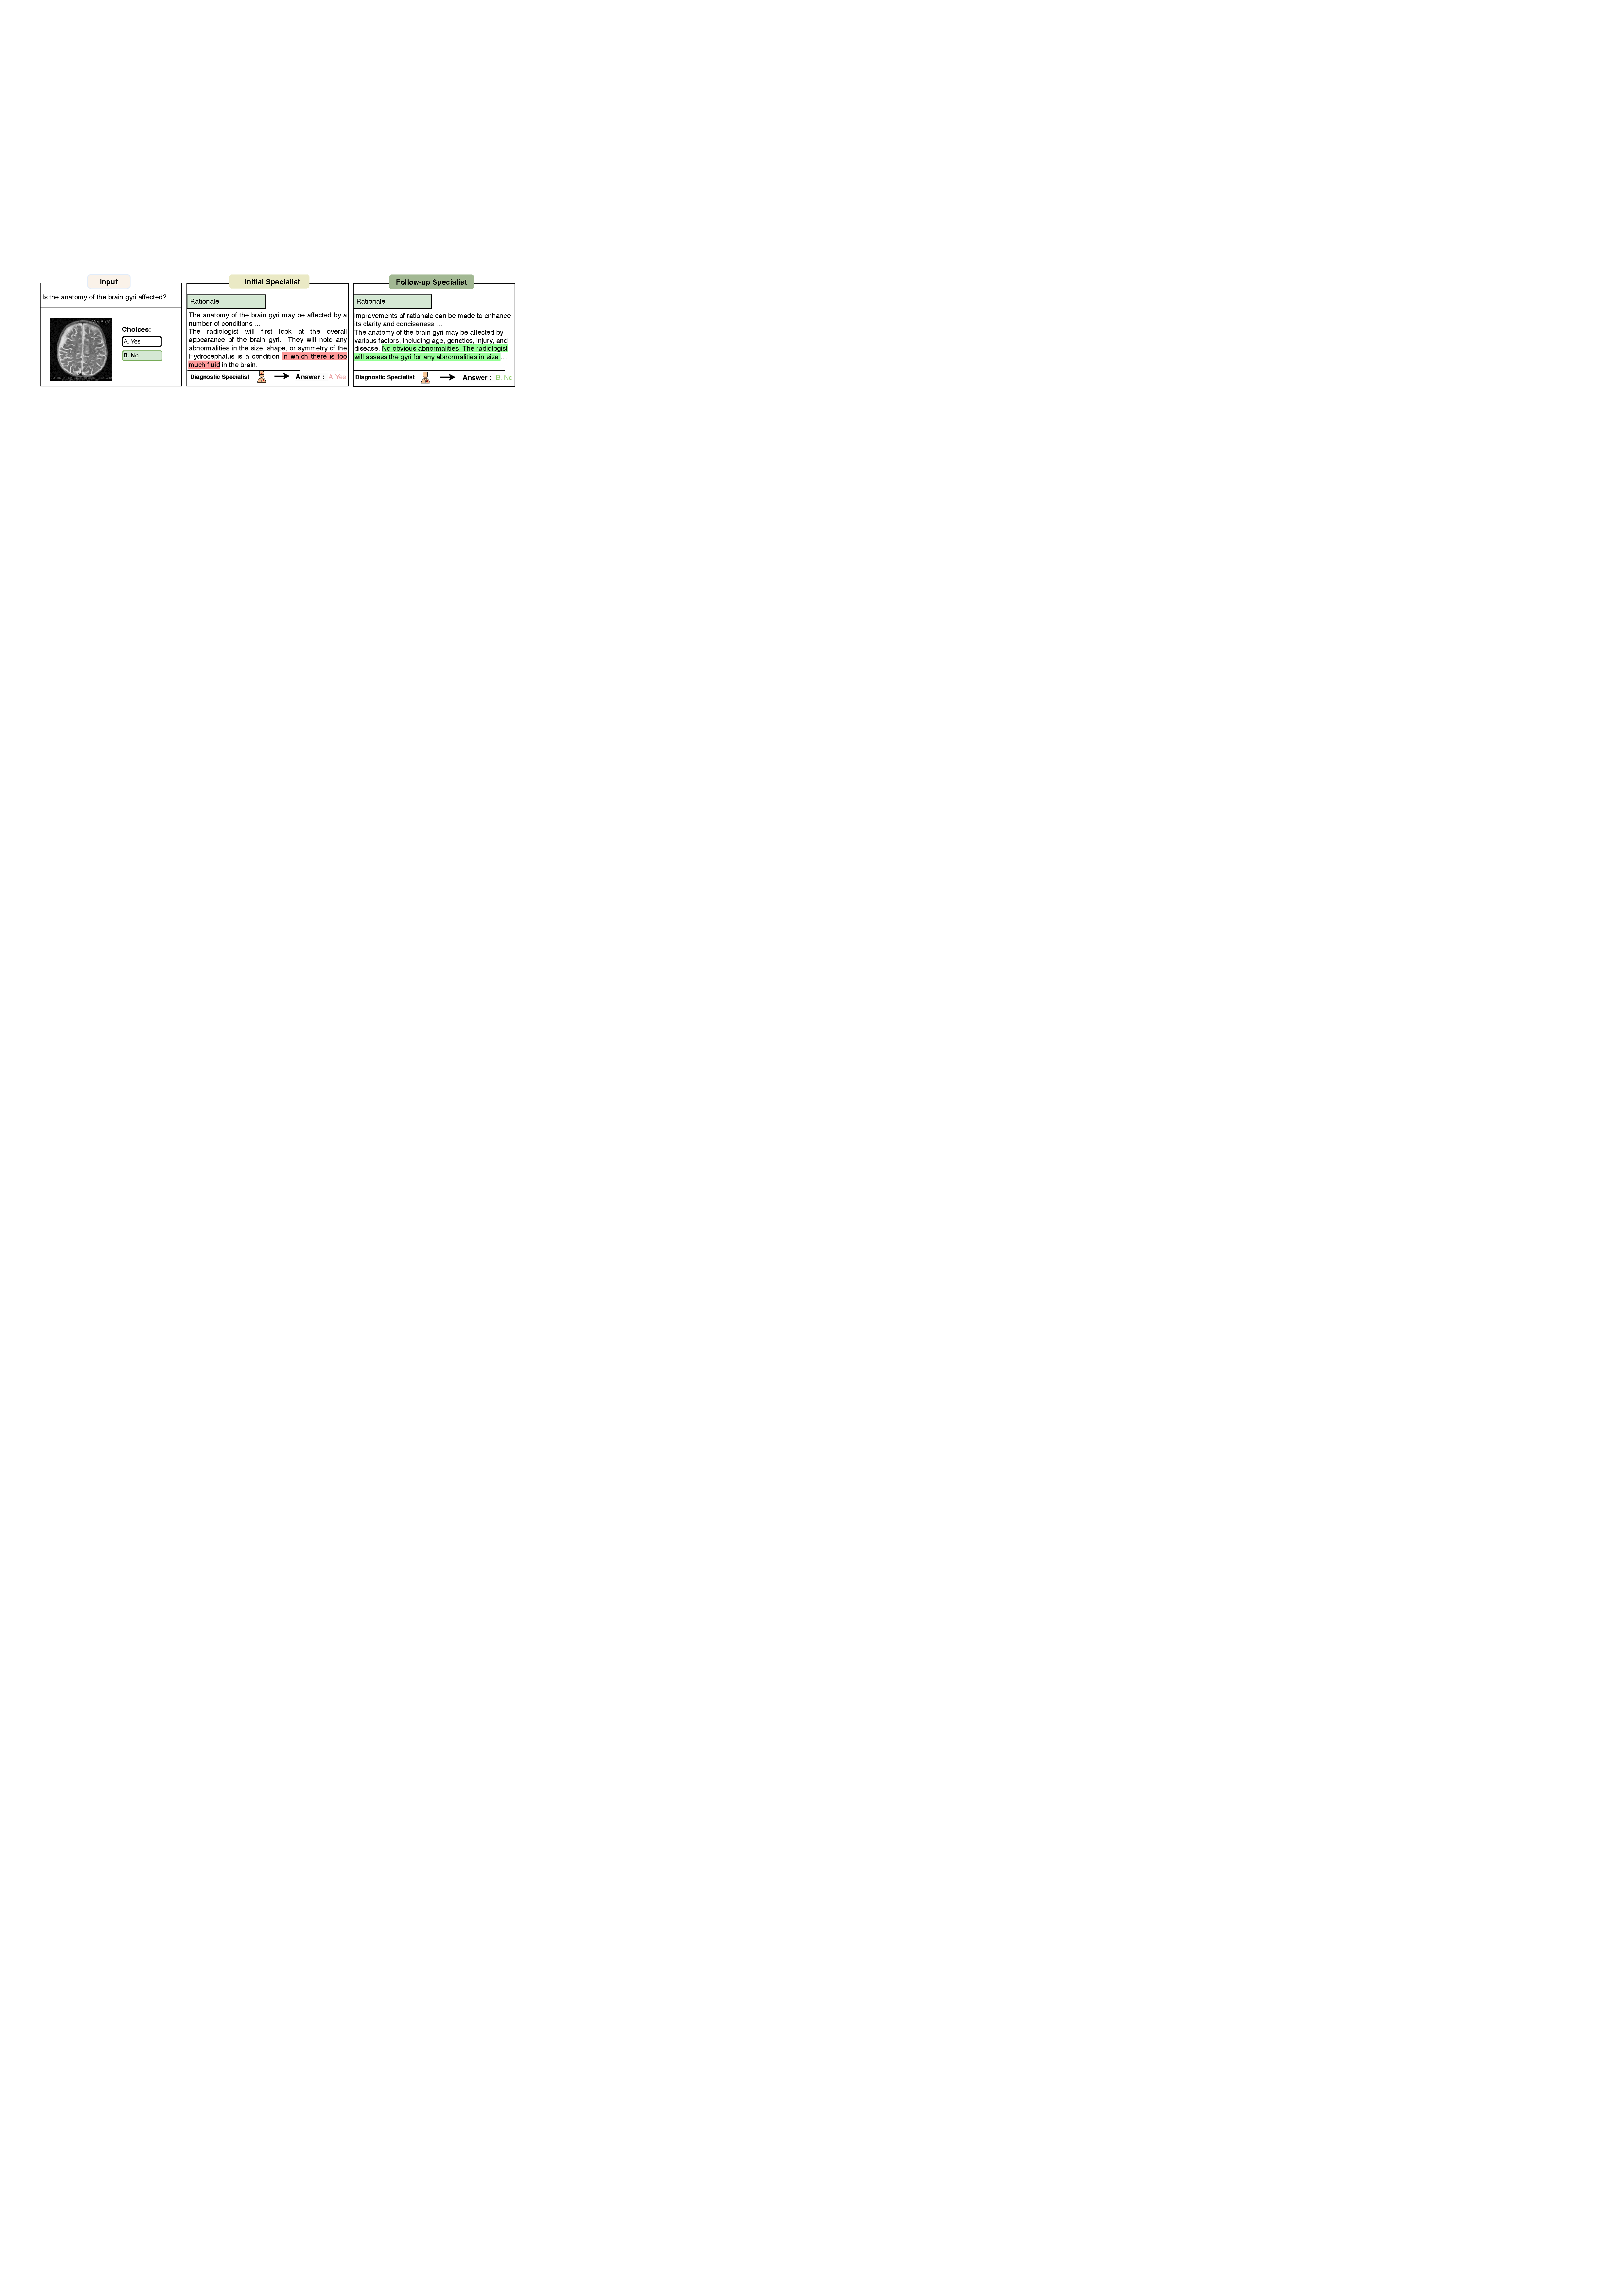
\includegraphics[width=\textwidth]{image/Figure_case1_v3.pdf}
% \caption{
% The MedCoT pipeline begins with an Initial Specialist receiving a medical question and image to generate a preliminary rationale. This rationale may have flaws (indicated in red), which are then reviewed by the Follow-up Specialist. If the rationale is deemed effective, it is retained; otherwise, it is reconsidered and a new rationale (indicated in green) is generated, along with an image caption. These elements are then integrated into the Diagnostic Specialist. Informed by all context, the Diagnostic Specialist, a multimodal language model with a designed sparse MoE structure, delivers the final diagnostic outcome (answer).
% } 
% \label{case1}
% \end{figure*}
% \vspace{-0.5em}
\subsection{Ablation Study}
\label{ablation}
\noindent\textbf{Effects of Follow-up Specialist}
To validate the effectiveness of the Follow-up Specialist, we compared the results of experiments involving only the initial and diagnostic specialists with those from the complete MedCoT. As shown in \autoref{xiaorong}, across two medical datasets, there is a significant performance loss when the Follow-up Specialist is removed. For instance, on the VQA-RAD dataset, performance dropped from 87.50\% to 80.88\%, a decrease of 6.62\%. This demonstrates the effectiveness of the Follow-up Specialist. 

Besides, we conducted experiments involving only the initial and diagnostic specialists, 
bypassing the self-reflection of the Follow-up Specialist. 
In all cases involving varying numbers of experts, the results without the self-reflection were consistently lower than those with rationales refined by the Follow-up Specialist’s reflection,  and even lower than those from a Diagnostic Specialist that had undergone self-reflection but was lacking the MoE component, as shown in \autoref{zhexiantu-all}. 
This underscores the importance of the self-reflection provided by the Follow-up Specialist.
%此外,我们也对Initial Specialist的rationale直接输入diagnostic Specialist进行了实验,缺少了Follow-up Specialist的自反思,在所有专家个数的情况下,都低于拥有自反思后的rationale的结果,甚至一直低于Follow-up自反思后的结果直接输入缺少MoE组件的diagnostic Specialist。证明了Follow-up Specialist带来的自反思的重要性。
Additionally, we conducted zero-shot experiments using both the initial and Follow-up Specialist. As shown in the appendix, these results further confirm the effectiveness of the Follow-up Specialist.

\noindent\textbf{Effects of MoE}
To validate the effectiveness of the MoE, we compared the performance with and without the MoE. As shown in \autoref{xiaorong}, there is a significant performance drop across all datasets without MoE. For instance, in the VQA-RAD, the performance decreased from 87.50\% to 82.72\%, a loss of 4.78\%. This indicates that MoE plays a crucial role in Diagnostic Specialist.
As can also be seen from \autoref{zhexiantu-all}, lacking MoE, in most expert number scenarios, the performance is weaker compared to MedCoT equipped with Sparse MoE.
%从Figure 3也可以看出,缺乏MoE,在大多数的expert number情况下,都弱于装载了Sparse MoE的MedCoT。
%此外,我们对于VQA-RAD和SLAKE-EN数据集中,每个部位都进行了实验,如Figure4和Figure5所示,可见,在绝大部分的器官的问题上,加载了MoE的方法都强于装载原始Gate的方法,值得一提的是,在VQA-RAD数据集的与Head器官相关的问题上,加载MoE的方法超过加载Gate方法10\%,近一步说明了MoE的效用,我们对Expert的权重进行可视化,如Figure4下图所示,可以看出,Expert 0和expert 5主要来处理相关Head器官的问题,说明了两个专家动态处理理解医学影像和文本的意图,强于原始的gate方法,可以称expert 0和expert 5为head专家。

Additionally, we conducted experiments for each organ-related question category within the VQA-RAD and SLAKE-EN, as shown in \autoref{rad}. 
It is evident that in the majority of organ-related questions, methods employing MoE outperform those using the gating mechanism. 
% Notably, Gate机制可以看作为一种单专家的形式,回答与Head-related的问题时,更容易出错(性能最低),for head-related questions in the VQA-RAD dataset, methods with MoE surpassed those with gates by 10\%, further underscoring the efficacy of MoE. 
% Notably, the Gate mechanism, akin to a single-expert system, is particularly prone to errors when addressing head-related questions, where it performs the worst. For head-related questions in the VQA-RAD dataset, MedCoT employing MoE surpassed those using gates by 10\%, further highlighting the efficacy of MoE.
Notably, the Gate mechanism, resembling as a single-expert system, tends to falter with head-related questions, where it performs the worst. For such questions in the VQA-RAD, methods using MoE exceeded those with gates by 10\%, further emphasizing MoE's effectiveness.
We visualized the weights of MoE, as shown in the \autoref{rad} (right figure), revealing that Experts 0 and 5 primarily handle head-related issues. This demonstrates that these two experts dynamically process and understand the intents of medical images and texts more effectively than the gating. 
% justifying the designation of Experts 0 and 5 as head specialists. 
Similar results can also be observed in the experiments conducted on the SLAKE-EN, as shown in Appendix.
%相似的结果也可以在Figure6中的slake-en数据集上的实验得出

% \noindent\textbf{Diagnostic Region Expert}

\noindent\textbf{Grid Search}
We conducted a parameter search experiment for the hyperparameters in the sparse MoE, such as the number of experts and the \( k \) value. The results are shown in Appendix. The experiment revealed that the optimal number of experts varies for different datasets. Specifically, the best number of experts for VQA-RAD, SLAKE-EN, Med-2019 and PathVQA are 6, 10, 5, and 5, respectively. Regarding the \( k \) value, the optimal value for all datasets was consistently 2, as illustrated in Appendix.
% \vspace{-0.5em}
\subsection{Discussion}
% \vspace{-0.5em}
% Three Case study
%Figure1和Figure2都展示了由初诊专家给出rationale,复诊专家进行纠正,诊断专家给出最终正确诊断结果的例子,如Figure5中,初诊专家在初诊中,受到大模型幻觉的干扰,导致观测到大脑中的不存在的brain fluid,因此诊断为brain受到gyri affected,而经过Follow-up Specialist的自反思,说明了没有明显观测到,最终诊断专家依据复诊专家的rationale综合上下文,得到了正确的诊断结果。
%Figure 3给出了一个例子,由于LLMs的能力有限,有些凭借大模型的能力不足以判断的cases,如Figure3中判断是否有pneumomediastinum?经过initial Specialist观测确定有,Follow-up认同了Initial Specialist的观点,得到了一致观点,然而由于LLms的能力不足,这些rationale错误,最终也导致了回答结果的错误。这也是MedCoT的一个限制:最终性能依赖于LLMs的能力。

\autoref{MedCoT pipeline} and \autoref{case1} illustrate cases where the Initial Specialist provides a rationale, the Follow-up Specialist makes corrections, and the Diagnostic Specialist delivers the final, accurate diagnosis. For instance, in \autoref{case1}, the Initial Specialist, influenced by the illusions of the LLMs, mistakenly observes non-existent brain fluid and diagnoses the brain as being affected by gyri. However, after the self-reflection by the Follow-up Specialist, it is clarified that no clear fluid was observed. Ultimately, the Diagnostic Specialist, using the rationale from the Follow-up Specialist and considering the full context, arrives at the correct diagnosis.

Appendix provides an example where the limitations of LLMs affect the ability to accurately diagnose certain cases. 
% In the scenario depicted in \autoref{case2}, 
The question posed is whether there is pneumomediastinum. The Initial Specialist, based on observations, affirms its presence, and the Follow-up Specialist concurs, leading to a unanimous agreement. However, due to the limitations of the LLMs, these rationales are incorrect, ultimately leading to an erroneous answer.


% \vspace{-0.5em}
\section{Conclusion}
% \vspace{-0.5em}
In this paper, we propose an effective hierarchical expert reasoning chain method for Med-VQA, named MedCoT. This method is based on two insights: 1) Med-VQA should have a clear reasoning path; 2) Med-VQA scenarios should be reviewed by multiple experts to arrive at a conclusion. Specifically, the process involves initial experts providing preliminary diagnostic rationales based on medical visual questions. Follow-up experts then review these rationales for validity, retaining the effective ones and reassessing the ineffective ones. Finally, a locally deployed Diagnostic Specialist, consisting of a sparse MoE that conducts a vote, then provides the definitive diagnosis. Experimental results on multiple Med-VQA datasets show that MedCoT outperforms existing SoTA techniques, significantly surpasses recent methods, and demonstrates excellent interpretability for final diagnosis.


\newpage
\section*{Limitation}
A limitation is that the performance of MedCoT is influenced by the hallucinations of the LLMs used by the Initial and Follow-up Specialist. 
Although self-reflection and Hierarchical Expert design can mitigate some issues with LLMs' hallucinations, it must be acknowledged that the problem is not completely resolved. As shown in Appendix, MedCoT is still susceptible to hallucination risks. Researching methods to suppress hallucinations is a potential topic for further study.
In this work, the Gemini-Pro model was employed. If Med-Gemini becomes available, MedCoT could be further enhanced.
Moreover, MedCoT could inspire future paradigms that integrate proprietary commercial LLMs with local models. 
By utilizing desensitized information to prompt the extensive knowledge and reasoning capabilities of LLMs, the generated rationales could be combined with local models for further diagnostic analysis, enhancing both interpretability and accuracy. 
% \autoref{case2} highlights a limitation of MedCoT: the final performance is partially dependent on the capabilities of the LLMs.
% 虽然自反思和Hierarchical Expert的设计可以缓解了部分的LLMs幻觉问题,但必须承认,这个问题并未完全解决。如图 \autoref{case2} 所示,MedCoT容易受到幻觉风险的影响。研究抑制幻觉的方法是进一步研究的潜在主题。

%由于我们的方法涉及零样本提示 LLM 以生成原理,因此存在从 LLM 继承社会偏见的潜在风险。这些偏见涵盖文化、道德和其他各个方面,可能会反映在生成的原理中,从而可能对用户产生不利影响。为了在未来缓解这个问题,潜在的解决方案可能涉及在每个提示阶段设计约束,或利用在无偏见资源上训练的更高级的 LLM。
Another limitation is that compared to single-model methods, MedCoT may be more time-consuming. However, the hierarchical expert approach aligns more closely with real-world medical diagnostics and provides clear diagnostic pathways as well as more accurate answers, making the additional time worthwhile.
% \subsection{Footnotes}
\section*{Acknowledgements}
This work is supported by the National Natural Science Foundation of China (Grant No. 62106222), the Natural Science Foundation of Zhejiang Province, China (Grant No. LZ23F020008), and the Zhejiang University-Angelalign Inc. R\&D Center for Intelligent Healthcare.
This work is also supported by Jiawei Du’s A*STAR Career Development Fund (CDF) C233312004.
% Footnotes are inserted with the \verb|\footnote| command.\footnote{This is a footnote.}

% \subsection{Tables and figures}

% See Table~\ref{tab:accents} for an example of a table and its caption.
% \textbf{Do not override the default caption sizes.}

% \begin{table}
%   \centering
%   \begin{tabular}{lc}
%     \hline
%     \textbf{Command} & \textbf{Output} \\
%     \hline
%     \verb|{\"a}|     & {\"a}           \\
%     \verb|{\^e}|     & {\^e}           \\
%     \verb|{\`i}|     & {\`i}           \\
%     \verb|{\.I}|     & {\.I}           \\
%     \verb|{\o}|      & {\o}            \\
%     \verb|{\'u}|     & {\'u}           \\
%     \verb|{\aa}|     & {\aa}           \\\hline
%   \end{tabular}
%   \begin{tabular}{lc}
%     \hline
%     \textbf{Command} & \textbf{Output} \\
%     \hline
%     \verb|{\c c}|    & {\c c}          \\
%     \verb|{\u g}|    & {\u g}          \\
%     \verb|{\l}|      & {\l}            \\
%     \verb|{\~n}|     & {\~n}           \\
%     \verb|{\H o}|    & {\H o}          \\
%     \verb|{\v r}|    & {\v r}          \\
%     \verb|{\ss}|     & {\ss}           \\
%     \hline
%   \end{tabular}
%   \caption{Example commands for accented characters, to be used in, \emph{e.g.}, Bib\TeX{} entries.}
%   \label{tab:accents}
% \end{table}

% As much as possible, fonts in figures should conform
% to the document fonts. See Figure~\ref{fig:experiments} for an example of a figure and its caption.

% Using the \verb|graphicx| package graphics files can be included within figure
% environment at an appropriate point within the text.
% The \verb|graphicx| package supports various optional arguments to control the
% appearance of the figure.
% You must include it explicitly in the \LaTeX{} preamble (after the
% \verb|\documentclass| declaration and before \verb|\begin{document}|) using
% \verb|\usepackage{graphicx}|.

% \begin{figure}[t]
%   \includegraphics[width=\columnwidth]{example-image-golden}
%   \caption{A figure with a caption that runs for more than one line.
%     Example image is usually available through the \texttt{mwe} package
%     without even mentioning it in the preamble.}
%   \label{fig:experiments}
% \end{figure}

% \begin{figure*}[t]
%   \includegraphics[width=0.48\linewidth]{example-image-a} \hfill
%   \includegraphics[width=0.48\linewidth]{example-image-b}
%   \caption {A minimal working example to demonstrate how to place
%     two images side-by-side.}
% \end{figure*}

% \subsection{Hyperlinks}

% Users of older versions of \LaTeX{} may encounter the following error during compilation:
% \begin{quote}
% \verb|\pdfendlink| ended up in different nesting level than \verb|\pdfstartlink|.
% \end{quote}
% This happens when pdf\LaTeX{} is used and a citation splits across a page boundary. The best way to fix this is to upgrade \LaTeX{} to 2018-12-01 or later.

% \subsection{Citations}

% \begin{table*}
%   \centering
%   \begin{tabular}{lll}
%     \hline
%     \textbf{Output}           & \textbf{natbib command} & \textbf{ACL only command} \\
%     \hline
%     \citep{Gusfield:97}       & \verb|\citep|           &                           \\
%     \citealp{Gusfield:97}     & \verb|\citealp|         &                           \\
%     \citet{Gusfield:97}       & \verb|\citet|           &                           \\
%     \citeyearpar{Gusfield:97} & \verb|\citeyearpar|     &                           \\
%     \citeposs{Gusfield:97}    &                         & \verb|\citeposs|          \\
%     \hline
%   \end{tabular}
%   \caption{\label{citation-guide}
%     Citation commands supported by the style file.
%     The style is based on the natbib package and supports all natbib citation commands.
%     It also supports commands defined in previous ACL style files for compatibility.
%   }
% \end{table*}

% Table~\ref{citation-guide} shows the syntax supported by the style files.
% We encourage you to use the natbib styles.
% You can use the command \verb|\citet| (cite in text) to get ``author (year)'' citations, like this citation to a paper by \citet{Gusfield:97}.
% You can use the command \verb|\citep| (cite in parentheses) to get ``(author, year)'' citations \citep{Gusfield:97}.
% You can use the command \verb|\citealp| (alternative cite without parentheses) to get ``author, year'' citations, which is useful for using citations within parentheses (e.g. \citealp{Gusfield:97}).

% A possessive citation can be made with the command \verb|\citeposs|.
% This is not a standard natbib command, so it is generally not compatible
% with other style files.

% \subsection{References}

% \nocite{Ando2005,andrew2007scalable,rasooli-tetrault-2015}

% The \LaTeX{} and Bib\TeX{} style files provided roughly follow the American Psychological Association format.
% If your own bib file is named \texttt{custom.bib}, then placing the following before any appendices in your \LaTeX{} file will generate the references section for you:
% \begin{quote}
% \begin{verbatim}
% \bibliography{custom}
% \end{verbatim}
% \end{quote}

% You can obtain the complete ACL Anthology as a Bib\TeX{} file from \url{https://aclweb.org/anthology/anthology.bib.gz}.
% To include both the Anthology and your own .bib file, use the following instead of the above.
% \begin{quote}
% \begin{verbatim}
% \bibliography{anthology,custom}
% \end{verbatim}
% \end{quote}

% Please see Section~\ref{sec:bibtex} for information on preparing Bib\TeX{} files.

% \subsection{Equations}

% An example equation is shown below:
% \begin{equation}
%   \label{eq:example}
%   A = \pi r^2
% \end{equation}

% Labels for equation numbers, sections, subsections, figures and tables
% are all defined with the \verb|\label{label}| command and cross references
% to them are made with the \verb|\ref{label}| command.

% This an example cross-reference to Equation~\ref{eq:example}.

% \subsection{Appendices}

% Use \verb|\appendix| before any appendix section to switch the section numbering over to letters. See Appendix~\ref{sec:appendix} for an example.

% \section{Bib\TeX{} Files}
% \label{sec:bibtex}

% Unicode cannot be used in Bib\TeX{} entries, and some ways of typing special characters can disrupt Bib\TeX's alphabetization. The recommended way of typing special characters is shown in Table~\ref{tab:accents}.

% Please ensure that Bib\TeX{} records contain DOIs or URLs when possible, and for all the ACL materials that you reference.
% Use the \verb|doi| field for DOIs and the \verb|url| field for URLs.
% If a Bib\TeX{} entry has a URL or DOI field, the paper title in the references section will appear as a hyperlink to the paper, using the hyperref \LaTeX{} package.

% \section*{Acknowledgments}

% This document has been adapted
% by Steven Bethard, Ryan Cotterell and Rui Yan
% from the instructions for earlier ACL and NAACL proceedings, including those for
% ACL 2019 by Douwe Kiela and Ivan Vuli\'{c},
% NAACL 2019 by Stephanie Lukin and Alla Roskovskaya,
% ACL 2018 by Shay Cohen, Kevin Gimpel, and Wei Lu,
% NAACL 2018 by Margaret Mitchell and Stephanie Lukin,
% Bib\TeX{} suggestions for (NA)ACL 2017/2018 from Jason Eisner,
% ACL 2017 by Dan Gildea and Min-Yen Kan,
% NAACL 2017 by Margaret Mitchell,
% ACL 2012 by Maggie Li and Michael White,
% ACL 2010 by Jing-Shin Chang and Philipp Koehn,
% ACL 2008 by Johanna D. Moore, Simone Teufel, James Allan, and Sadaoki Furui,
% ACL 2005 by Hwee Tou Ng and Kemal Oflazer,
% ACL 2002 by Eugene Charniak and Dekang Lin,
% and earlier ACL and EACL formats written by several people, including
% John Chen, Henry S. Thompson and Donald Walker.
% Additional elements were taken from the formatting instructions of the \emph{International Joint Conference on Artificial Intelligence} and the \emph{Conference on Computer Vision and Pattern Recognition}.

% Bibliography entries for the entire Anthology, followed by custom entries
%\bibliography{anthology,custom}
% Custom bibliography entries only
\bibliography{main}
\newpage

% \appendix

% \section*{Appendix}
% \label{sec:appendix}
% In this section, we present additional implementation details, experiment results, and supplements. The content structure is outlined as follows:

% \begin{itemize}[itemsep=0pt, parsep=0pt]
%     \item Section~\ref{secA} - MedCoT on Four Datasets 
%     % \item Section~\ref{gate} - Gate
%     \item Section~\ref{supmethod} - Method Details
%     \begin{itemize}
%         \item Section~\ref{gate} - Gate Mechanism
%         \item Section~\ref{secB2} - MedCoT Method Details
%     \end{itemize}
%     \item Section~\ref{secD} - Datasets
%     \item Section~\ref{secE} - The Effect of Initial Specialist
%     \item Section~\ref{secF} - Self-Reflection in Follow-up Specialist
%     \begin{itemize}
%         \item Section~\ref{secF1} - Effectiveness of Self-Reflection in Follow-up Specialist
%         \item Section~\ref{secF2} - Error Analysis on Self-Reflection
%     \end{itemize}
%     \item Section~\ref{secH1} - Computing Resource Costs
%     \item Section~\ref{secH2} - Assessing the Impact of Different Prompts
%     \item Section~\ref{secG} - Prompt Template
% \end{itemize}

% % \usepackage{multirow}
% % \usepackage{booktabs}

% % \usepackage{booktabs}


% \begin{table*}
% \centering
% \caption{Comparison of model performances across different datasets on closed-end question: All results are in \%, the best ones are in \textbf{bold}.}
% \label{maintable}
% \resizebox{\linewidth}{!}{
% \begin{tabular}{cccccc} 
% \toprule
% Model          &Size         & VQA-RAD        & SLAKE-EN       & VQA-Med 2019   & PathVQA         \\ 
% \midrule

% {CGMVQA Ens.} \cite{ren2020cgmvqa}      & -       & -              & -              & 78.10          & -               \\
% {MEVF} \cite{nguyen2019overcoming}        & -           & 77.20          & 79.80          & -              & -               \\
% {MMBERT} \cite{khare2021mmbert}       & -          & 77.90          & -              & 78.10          & -               \\
% {WDAN} \cite{huang2023dual}        & -           & 76.50          & -              & 81.20          & -               \\
% Gemini Pro \cite{qi2023gemini}     & -         & 60.29          & 72.60          & 60.22              & 70.30              \\
% {PubmedCLIP} \cite{eslami-etal-2023-pubmedclip}     & -        & 79.50          & 82.50          & -              & -               \\
% {VL Encoder-Decoder} \cite{bazi2023vision}  & -  & 82.47          & -              & -              & 85.61           \\
% {Q2ATransformer} \cite{liu2023q2atransformer}    & -     & 81.20          & -              & -              & 88.85           \\
% {VQA-Adapter} \cite{liu2023parameter}     &  -        & 82.30          & 83.70          & -              & -               \\
% MedThink \cite{gai2024medthink}      &  223M        & 83.50          & 86.30          & -              & -               \\
% Prefix T \cite{van2023open}      & 1.5B          & -              & 82.01          & -              & 87.00           \\
% LLaVA \cite{li2024llava}      &   7B          & 65.07          & 63.22          & -              & 63.20           \\
% LLAVA-Med (From LLaVA) \cite{li2024llava} &7B  & 84.19          & 85.34          & -              & 91.21           \\
% LLaVA-Med (From Vicuna) \cite{li2024llava} &7B  & 81.98          & 83.17          & -              & \textbf{91.65}  \\
% LLAVA-Med (BioMed CLIP) \cite{li2024llava} &7B & 83.09          & 86.78          & -              & 91.09           \\ 
% \hline\hline
% MedCoT (Ours)   &    $ \sim $ 256M    & \textbf{87.50} & \textbf{87.26} & \textbf{82.81} & 90.37           \\
% \bottomrule
% \end{tabular}
% }
% \end{table*}


% \begin{table*}
% \centering
% \small
% \caption{Evaluation Metrics for SLAKE-EN and VQA-RAD on Open-end datasets.}
% \label{open}
% \begin{tabular}{cccccc} 
% \toprule
%                           &               & Rouge1         & Rouge-L        & Rouge-Lsum     & BLEU-1          \\ 
% \midrule
% \multirow{2}{*}{SLAKE-EN} & MedCoT (ours) & \textbf{80.86} & \textbf{80.14} & \textbf{80.12} & \textbf{78.33}  \\
%                           & MedThink      & 80.12          & 79.91          & 79.93          & 77.94           \\
% \multirow{2}{*}{VQA-RAD}  & MedCoT (ours) & \textbf{66.30} & \textbf{65.78} & \textbf{65.98} & \textbf{61.29}  \\
%                           & MedThink      & 58.10          & 58.09          & 58.10          & 51.76           \\
% \bottomrule
% \end{tabular}
% \end{table*}


% \begin{figure*}
% \centering
% 
\includegraphics[width=\textwidth]{image/Figure_case2.pdf}
% \caption{
% The MedCoT pipeline begins with an Initial Specialist receiving a medical question and image to generate a preliminary rationale. This rationale may have flaws (indicated in red), which are then reviewed by the Follow-up Specialist. If the rationale is deemed effective, it is retained; otherwise, it is reconsidered and a new rationale (indicated in green) is generated, along with an image caption. These elements are then integrated into the Diagnostic Specialist. Informed by all context, the Diagnostic Specialist, a multimodal language model with a designed sparse MoE structure, delivers the final diagnostic outcome (answer).
% } 
% \label{case2}
% \end{figure*}


% \begin{figure*}[t]
% \centering
% 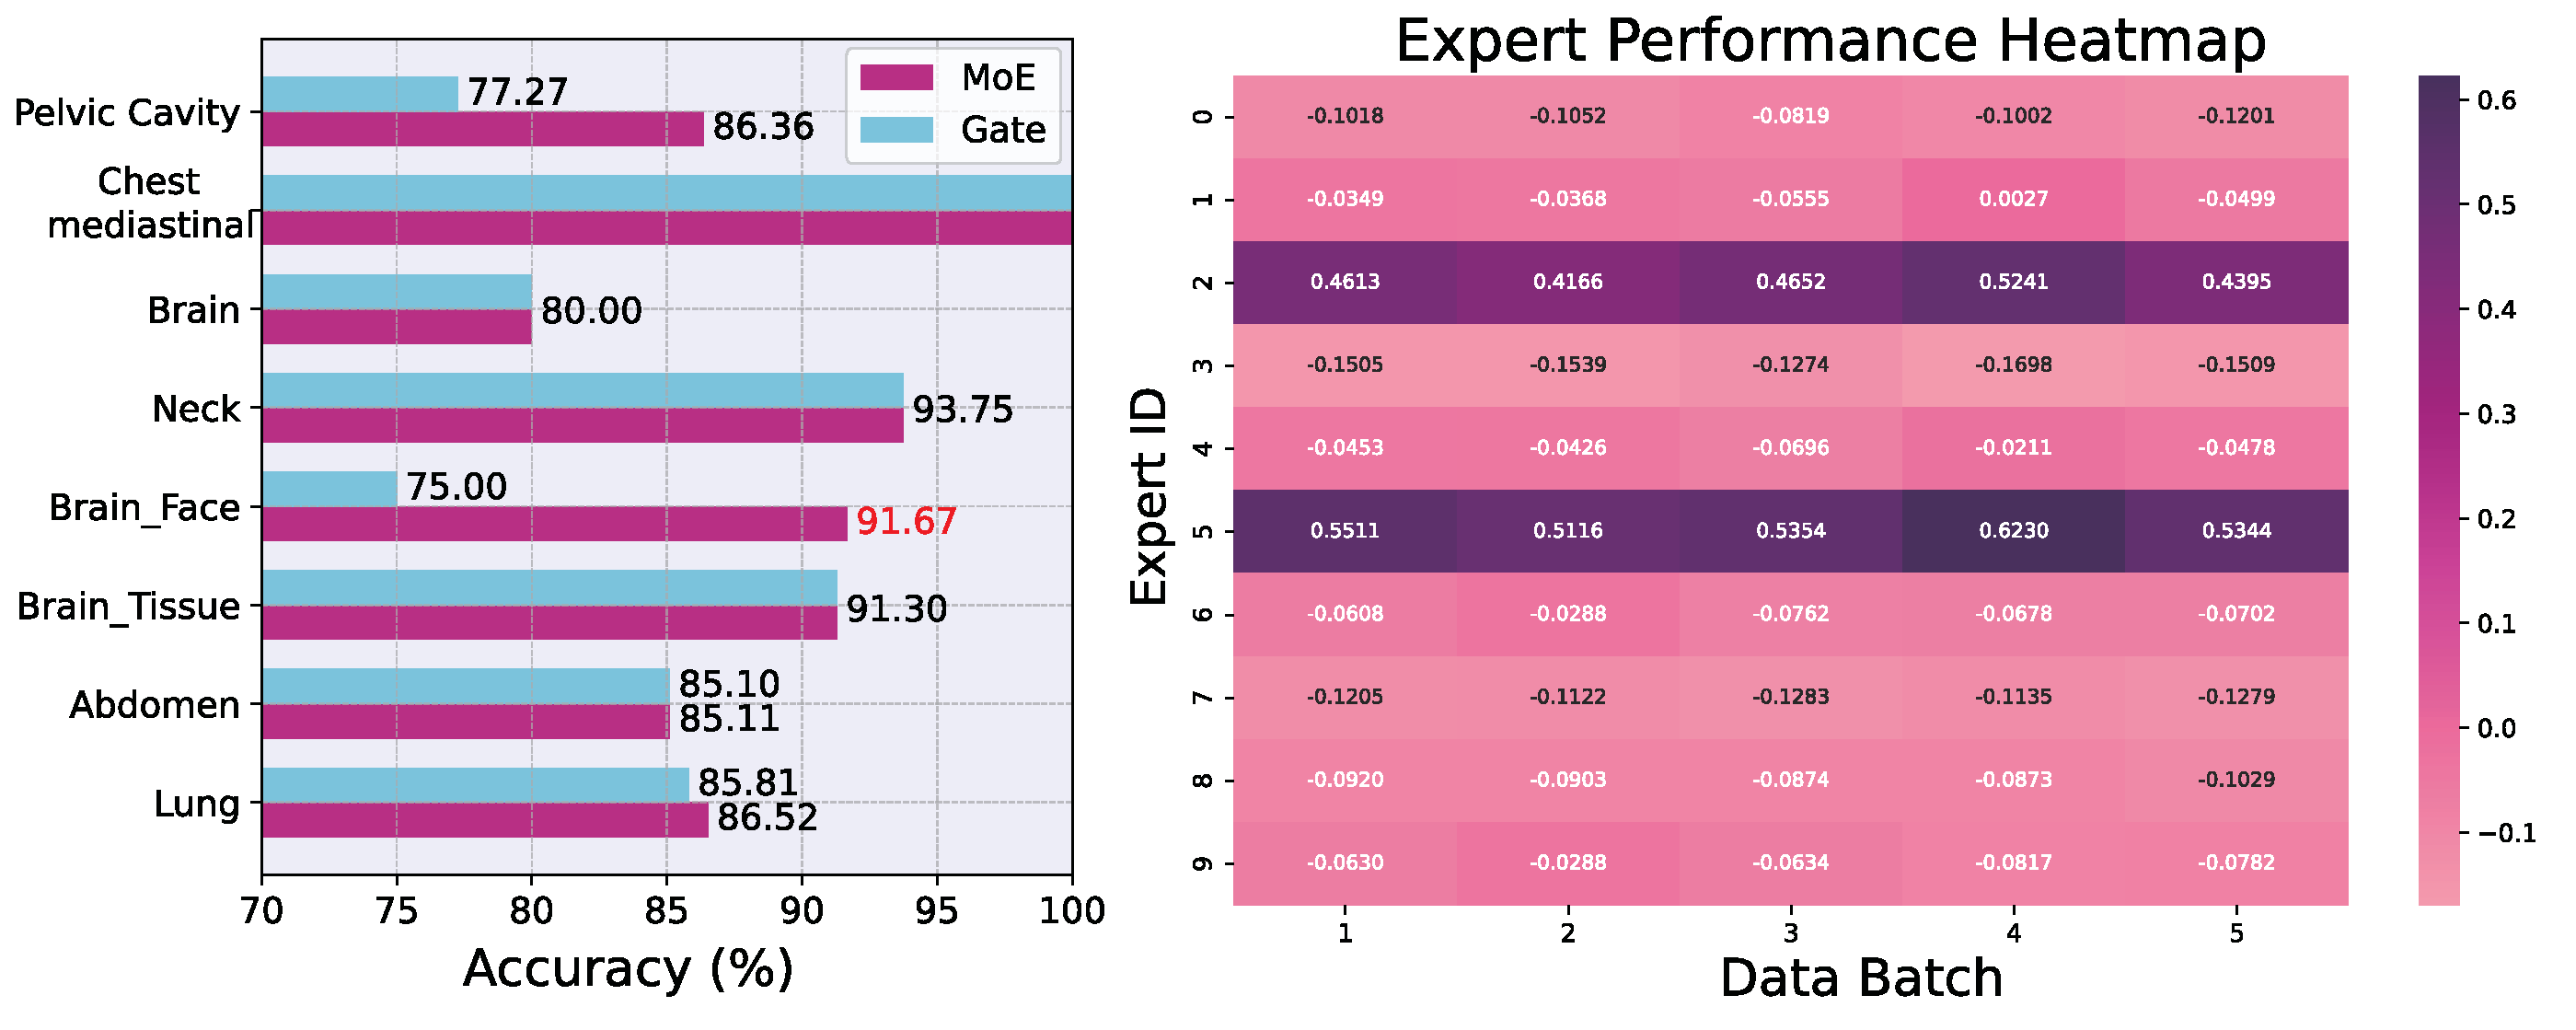
\includegraphics[width=\textwidth]{image/SLAKE-v2.pdf}
% \caption{
% The Diagnostic Specialist's sparse MoE demonstrates varying accuracy levels for different organ-related questions in the SLAKE-EN dataset.
% It can be observed that questions related to "Brain Face" organs saw an improvement of nearly 16 \%. We visualized the weights of the experts (right figure). Notably, in the top 2 expert selections, the model chose Expert 2 and Expert 5 to understand the intents of the "face" image and text. Experts 2 and 5 can be considered as "Face" specialists, proficient in diagnosing issues related to "Face".
% } 
% \label{slake}
% \end{figure*}


% \begin{figure*}[ht!]
% \centering
% 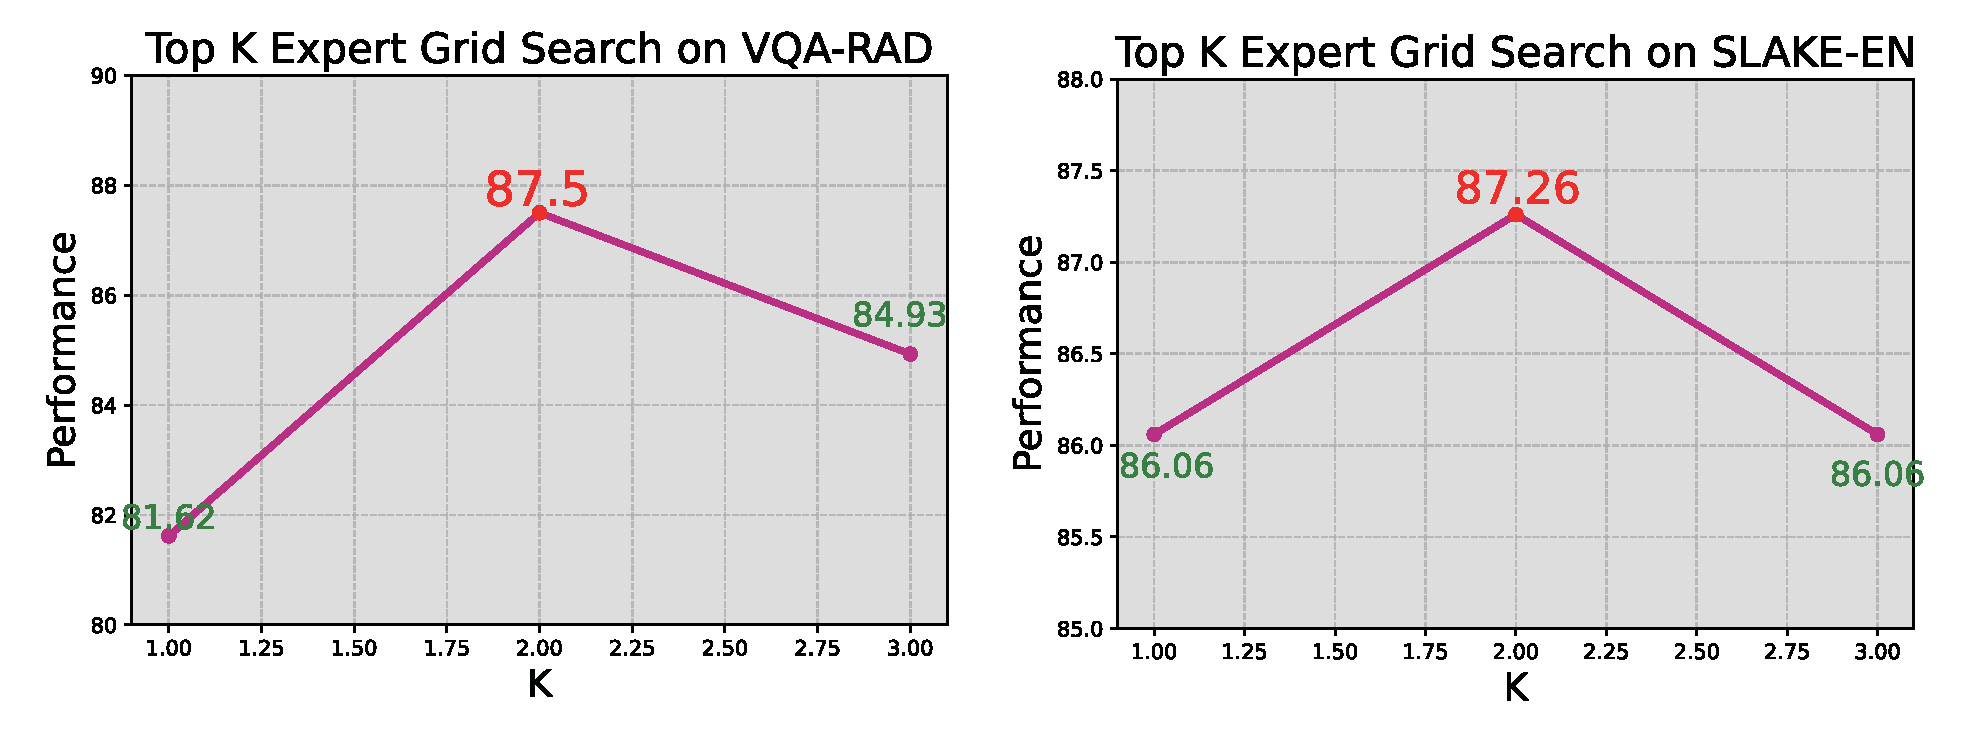
\includegraphics[width=\textwidth]{image/zhexiantu-v4.pdf}
% \caption{
% The top $k$ expert grid search experiment on the VQA-RAD and SLAKE-EN.
% } 
% \label{zhexiantu_k}
% \end{figure*}

% \begin{figure*}[t]
% \centering
% 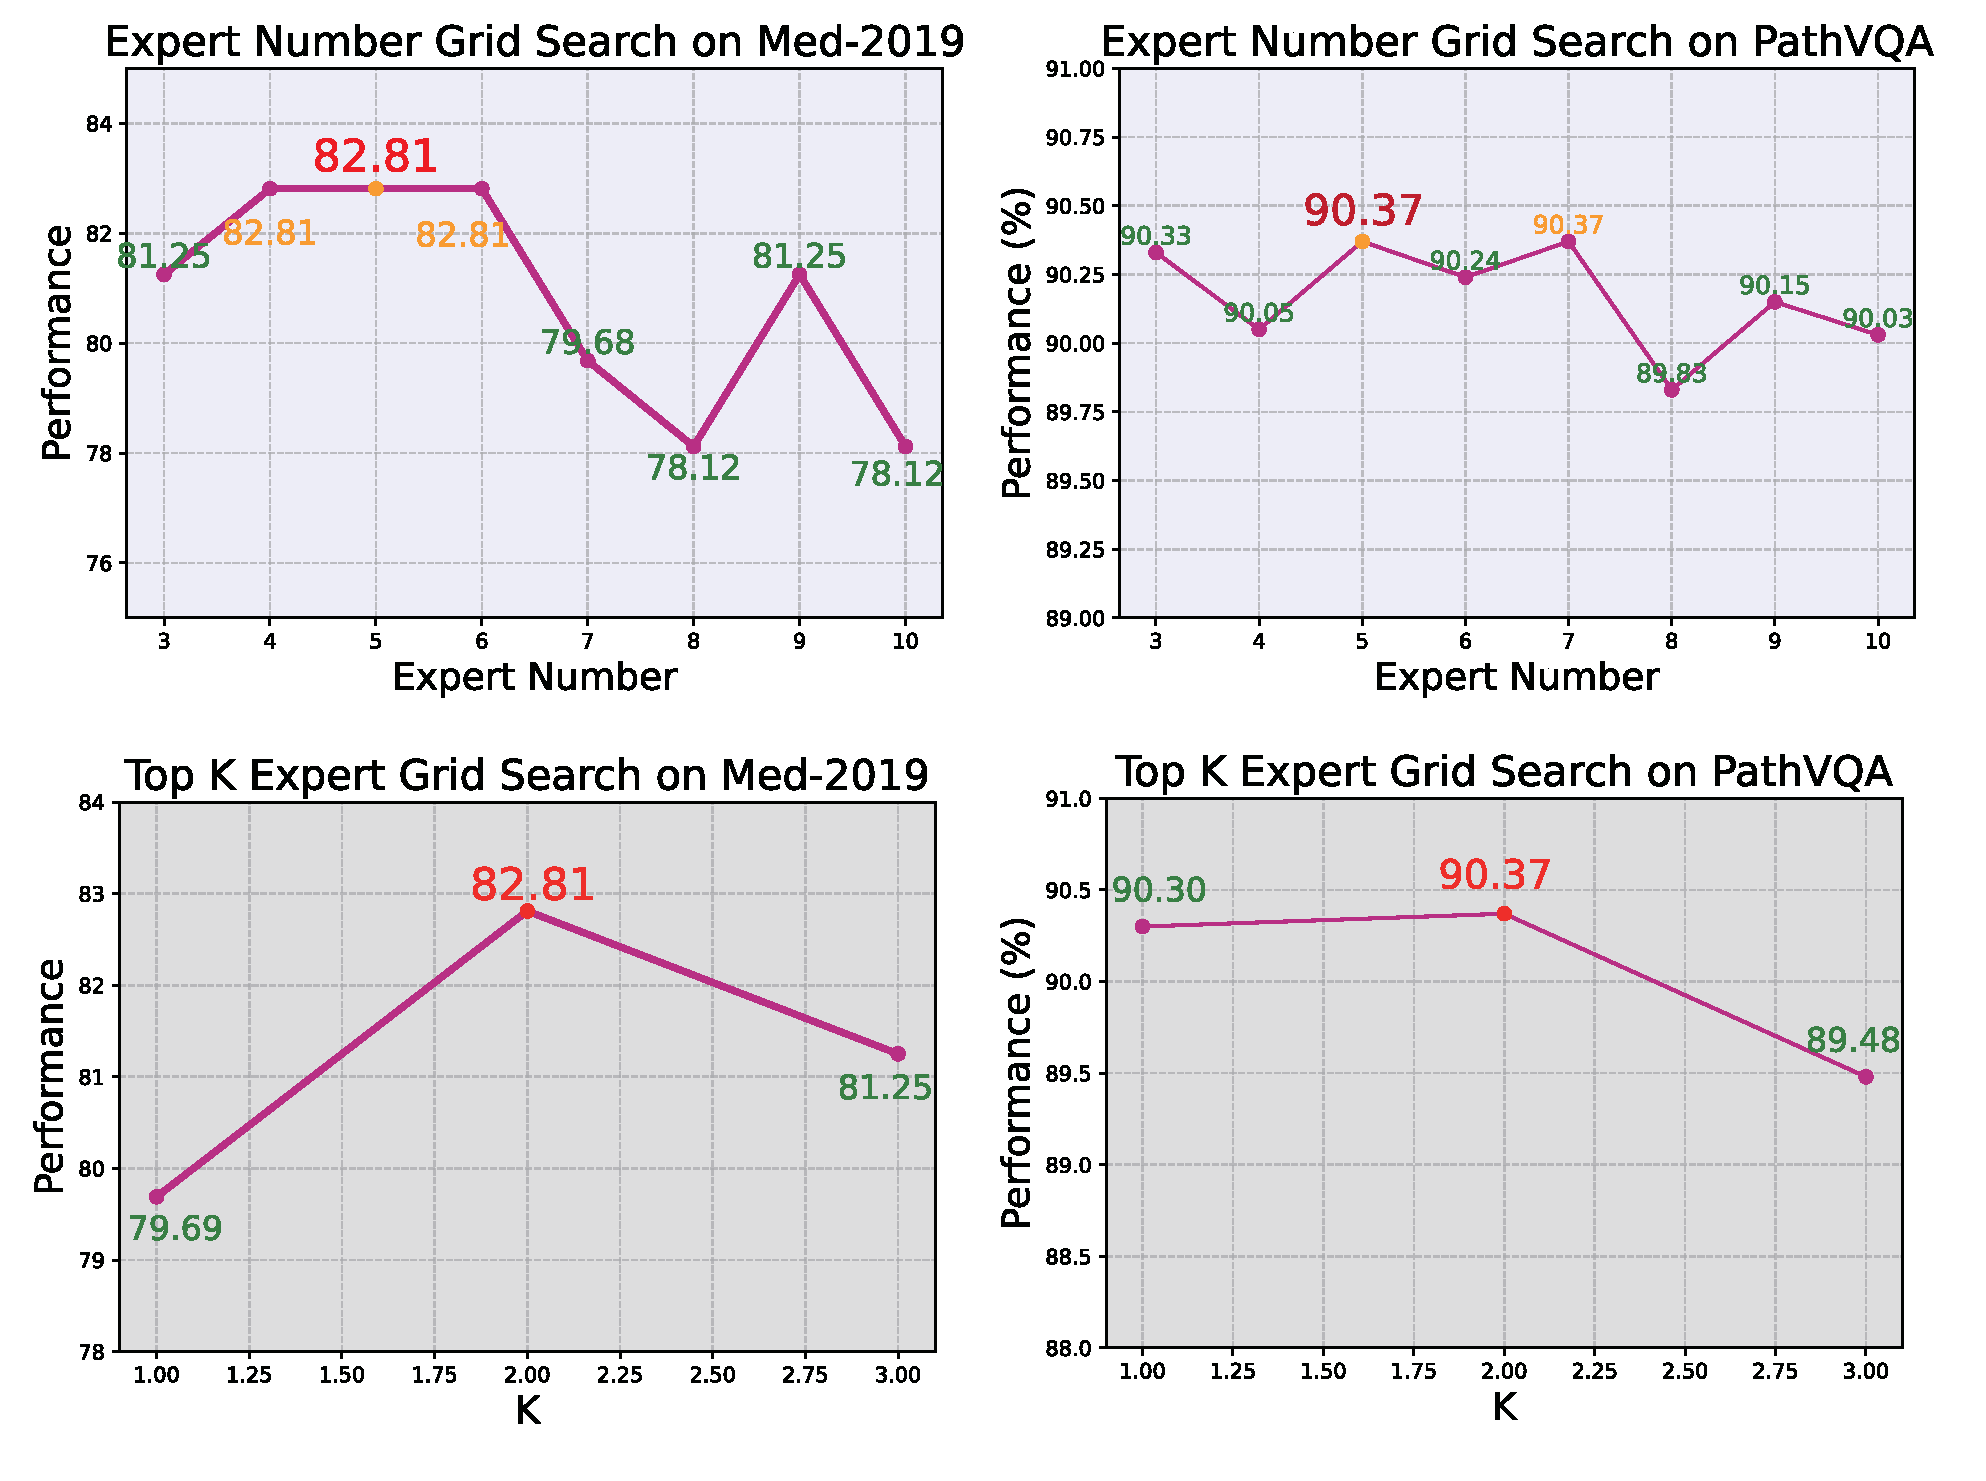
\includegraphics[width=\textwidth]{image/zhexiantu-change.pdf}
% \caption{
% In the Expert Number grid search experiment on the Med-VQA-2019 and PathVQA, the purple line represents results from using rationales provided by the Follow-up Specialist and grid searching expert numbers in the Diagnostic Specialist thereafter (upper figure). 
% The top $k$ expert grid search experiment on the Med-VQA-2019 and PathVQA (lower figure).
% } 
% \label{pathvqa}
% \end{figure*}

% \section{MedCoT on Four Datasets}
% \label{secA}
% \autoref{maintable} presents a comparison of methods performances across various datasets on closed-end questions. MedCoT, not only achieves superior performance but also demonstrates significant efficiency in model size compared to SoTA models. Despite being more lightweight, MedCoT consistently outperforms larger models across different datasets.
% \begin{itemize}
%     \item \textbf{Efficiency in Size}: MedCoT has a model size of $\sim$256M, which is significantly smaller than many other models such as Prefix T (1.5B), and LLAVA variants (7B). Note that the MedCoT model has approximately 256M parameters with 5 experts, 257M with 6 experts, and 261M with 10 experts.
%     \item \textbf{Superior Performance}: Despite its smaller size, MedCoT achieves the highest or near-highest scores across multiple datasets, with notable performance on VQA-RAD (87.50\%), SLAKE-EN (87.26\%), VQA-Med 2019 (82.81\%), and PathVQA (90.37\%). 
%     For example, on the VQA-RAD dataset, MedCoT improved by 27.21\% over Gemini and achieved a 3.31\% increase compared to the strongest performance of LLaVA, which has 7B training parameters and was trained on extensive medical data. These results indicate that our self-reflection and Hierarchical Expert design effectively reduce errors and ensure the accuracy of multimodal reasoning in LLMs.
%     % 例如,在VQA-RAD上,MedCoT在比Gemini提高了 27.21\%,与训练参数7B的LLaVA(训练了大量医学数据)最强性能相比,提升了3.31\%,这些表明,我们的自反思和Hierarchical Expert的设计能够有效地减少了错误,保证了 LLM 中多模态推理的准确性。
%     Open-end questions allow for a range of answers due to their inherent nature. The answers generated by MedCoT are difficult to match precisely against the dataset. Therefore, we employ text generation metrics such as Rouge and BLEU to evaluate MedCoT's performance, as exhibited in \autoref{open}.
% We conducted experiments on the open-end VQA-RAD and SLAKE-EN, with results shown in the Appendix \autoref{open}. 
% The Rouge score, similar to "recall," emphasizes the completeness of the generated text, while the BLEU score, akin to "precision," highlights its accuracy. 
% MedCoT demonstrated higher Rouge and BLEU scores on the VQA-RAD dataset, with Rouge-1 and BLEU-1 reaching 66.30\% and 61.29\%, respectively, surpassing MedThink \cite{gai2024medthink}. Besides, MedCoT also showed higher scores on the SLAKE-EN.
% \end{itemize}


% \section{Method Details}
% \label{supmethod}

% \subsection{Gate Mechanism}
% \label{gate}
% The \textit{Gated Dense Layer} fuses the textual representation \( F_T \) and the attention-guided visual feature \( H_{V}^{\text{att}} \), deriving the fusion coefficient \( \lambda \) through a sigmoid-activated linear combination of these modalities:
% \begin{align}
%          \lambda &= \text{Sigmoid}(W_lF_T + W_vH_{V}^{\text{att}}),
% \end{align}
% where $W_l$ and $W_v$ are the model parameters learned during training which optimize the blend of information from the textual and visual streams. The integrated output $F_{\text{I}} \in\mathbb{R}^{n \times d}$ is then computed as a weighted sum of $F_T$ and $H_{V}^{att}$, moderated by $\lambda$:
% \begin{align}
%     F_{\text{I}} &= (1-\lambda) \cdot F_{\text{T}} + \lambda \cdot H_{V}^{\text{att}}.
% \end{align}


% The gate $\lambda \in [0,1]$ is to weight the expected importance of image for source text. The gate dense layer is trainable. $W_l$ and $W_v$ are the learnable parameters to fuse the input $F_T \in \mathbb{R}^{n \times d}$ and $H_V^{\text{att}} \in \mathbb{R}^{n \times d}$ for output $F_l$. 

% % This is an appendix.



% \subsection{MedCoT Method Details}
% \label{secB2}
% For Diagnostic Specialist, we adopt the Flan-T5 encoder-decoder architecture in its Base version. The loss function is configured in accordance with the settings from T5 \cite{zhang2023multimodal}. 
% The dimension of the vision features (processed by VisualEncoder DETR: $detr_{resnet101 dc5}$) is (100,256)).

% \section{Datasets}
% \label{secD}
% Four well-known Med-VQA datasets are used in MedCoT: VQA-RAD \cite{lau2018dataset}, SLAKE-EN \cite{liu2021slake}, VQA-2019\cite{abacha2019vqa}, and PathVQA \cite{he2020pathvqa}. 
% Each question and Image can be classified into closed-end questions and open-end questions (see \autoref{tab:datasets}).

% % \usepackage{booktabs}


% % \begin{table}[htbp]
% % \centering
% % \caption{\label{}Details on datasets: The distribution of the closed-end and open-end attributes of question in the four data sets.  }
% % \resizebox{\linewidth}{!}{
% % \begin{tabular}{llrr}
% % \toprule
% % Dataset  & Modality & Source &  Images &  QA pairs \\
% % \midrule
% % VQA-RAD~\cite{lau2018dataset} &  Radiology  & 0.3k & 3.5k\\
% % PathVQA~\cite{he2020pathvqa} &  Pathology  & 5k & 32.8k  \\
% % SLAKE-EN~\cite{liu2021slake} & Radiology  & 0.7k & 14k  \\
% % VQA-2019~\cite{ben2021overview} & Radiology &  5k & 5k\\
% % \bottomrule
% % \end{tabular}}
% % \label{tab:datasets}
% % \end{table}

% \begin{table}[htbp]
% \centering
% \caption{\label{tab:datasets}Details on datasets: The distribution of the closed-end and open-end attributes of questions in the four datasets.}
% \resizebox{\linewidth}{!}{
% \begin{tabular}{l  r r}
% \toprule
% Dataset  & Images & QA pairs \\
% \midrule
% VQA-RAD~\cite{lau2018dataset}  & 0.5k & 3.5k \\
% PathVQA~\cite{he2020pathvqa}  & 5k & 32.8k \\
% SLAKE-EN~\cite{liu2021slake}  & 0.7k & 14k \\
% VQA-2019~\cite{Abacha2019VQAMedOO}  & 5k & 13k \\
% \bottomrule
% \end{tabular}
% }
% \end{table}









% \section{The Effect of Initial Specialist}
% \label{secE}
% To evaluate the effect of Initial Specialist, we randomly sampled 100 question sets that had undergone Initial Specialist CoT prompting. 
% These sets were then assembled into <Question, Options, Rationale, Answer> quadruples. 
% Initial Specialist demonstrated robust performance across these quadruples, indicating that the CoT approach enhances the performance of MedVQA (see \autoref{tab:Verifying CoT Utility}).

% Besides, to validate the generalization efficacy of Initial Specialist, we randomly sampled data from four datasets to construct a validation set. The results, presented in \autoref{tab:Verifying CoT Utility}, provide empirical evidence supporting the robustness and effectiveness in Initial Specialist. 


% \begin{table}[htbp]
% \caption{\label{}
% Verifying CoT Utility: The ability of large models guided by CoT in MedVQA
%   }
% \resizebox{\linewidth}{!}{
% \begin{tabular}{cccccc}
% \hline
% \textbf{}                                                                        & \textbf{VQA-RAD} & \textbf{SLAKE-EN} & \textbf{VQA-2019} & \multicolumn{1}{l}{\textbf{PathVQA}} & \multicolumn{1}{l}{\textbf{Mixture Set}} \\ \hline
% \begin{tabular}[c]{@{}c@{}}Zero-shot prompting \\ with rationale\end{tabular} & 72               & 70                & 68                & 76                                   & 73                                       \\ \cline{1-1}
% \begin{tabular}[c]{@{}c@{}}Zero-shot prompting \\ without rationale\end{tabular}    & 47               & 44                & 37                & 49                                   & 46                                       \\ \hline
% \end{tabular}
% }
% \end{table}

% \usepackage{booktabs}


% \begin{table*}
% \centering
% \caption{Verifying Initial Specialist Utility. The numbers in the table represent the count of correctly answered questions out of the 100 sampled.}
% \resizebox{\linewidth}{!}{
% \begin{tabular}{cccccc} 
% \toprule
% \textbf{}                                                                        & {VQA-RAD} & {SLAKE-EN} & {VQA-2019} & {PathVQA} & {Mixture Set}  \\ 
% \hline
% \begin{tabular}[c]{@{}c@{}}Initial Specialist CoT prompting \end{tabular}    & 72               & 70                & 68                & 76               & 73                    \\
% \begin{tabular}[c]{@{}c@{}}LLMs prompting  w/o rationale\end{tabular} & 47               & 44                & 37                & 49               & 46                    \\
% \bottomrule
% \end{tabular}
% }
% \label{tab:Verifying CoT Utility}
% \end{table*}





% \section{Self-Reflection in Follow-up Specialist}
% \label{secF}
% Self-Reflection, introduced \cite{shinn2023reflexion,xu2024preemptive}, is a technique initially designed to assist LLMs like Gemini Pro/GPT-4 in addressing hallucinations and optimizing planning. 
% % It involves prompting the model to self-assess its outputs and identify potential fallacies. This concept is akin to metacognition in humans, where individuals reflect on their thought processes to improve learning and problem-solving abilities. Key aspects of self-reflection in LLMs include error detection and correction, reasoning and justification, performance metrics, learning from mistakes, user interaction feedback, and knowledge updates. For error detection, models analyze their responses post-generation to identify inconsistencies, implementing feedback loops to refine future outputs. Reasoning and justification are enhanced by encouraging models to explain their reasoning and generate self-questions to verify accuracy.
% Self-Reflection in LLMs, akin to human metacognition, involves the model self-assessing its outputs to identify and correct errors, enhance reasoning and justification, and integrate feedback and knowledge updates, thereby improving learning and problem-solving capabilities.

% \subsection{Effectiveness of Self-Reflection in Follow-up Specialist}
% \label{secF1}
% To better demonstrate the impact of model self-reflection on the quality of rationales and its influence on the final answer judgment, we employed a zero-shot prompting method. By forming <Question, Options, Rationale, Answer> quadruples as prompts and utilizing the Gemini-pro-1.5 API for evaluation, we obtained the data presented in \autoref{zeroshot-self}. 
% The Follow-up Specialist, by employing Self-Reflection after the Initial Specialist, achieves significant improvements in the accuracy of closed-end questions across the majority of the four datasets.

% % \begin{table*}[htbp]
% % \caption{\label{}
% % Verifying CoT Utility: The ability of large models guided by CoT in MedVQAModel performance in Zero-shot condition
% %   }
% %   \centering
% % % \resizebox{\linewidth}{!}{
% % \begin{tabular}{ccccc}
% % \hline
% % \centering
% % \textbf{}        & {VQA-RAD} & {SLAKE-EN} & {VQA-2019} & \multicolumn{1}{l}{{PathVQA}} \\ \hline
% % Zero-shot (Initial specialist) & 59.56            & 73.07             & 59.79             & 65.63                                \\
% % Zero-shot (Follow-up specialist) & 60.29            & 72.60             & 60.22             & 70.30                                \\ \hline
% % \end{tabular}
% % % }
% % \end{table*}

% \begin{figure}[htbp]
% \centering
% 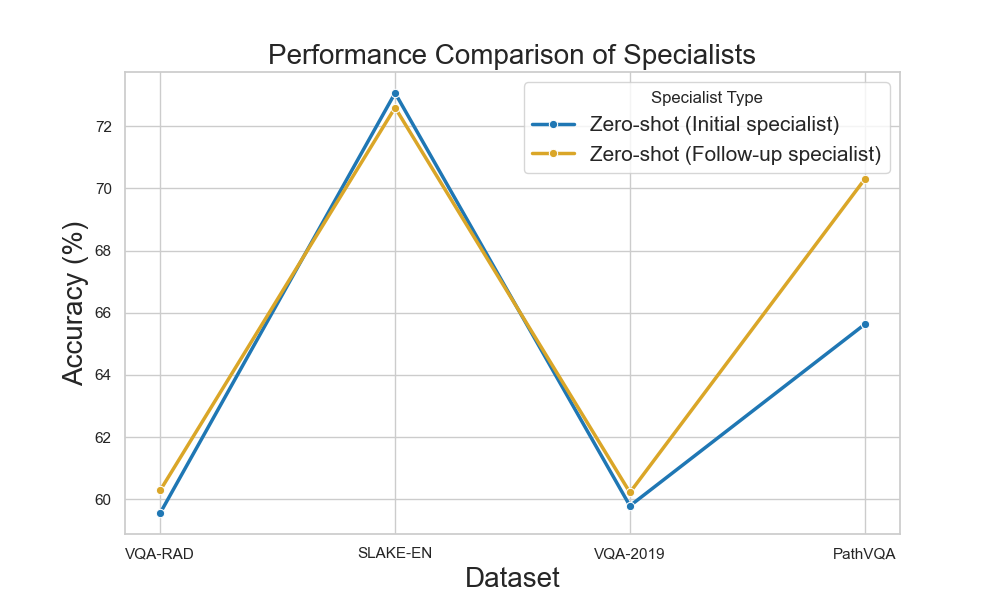
\includegraphics[width=0.5\textwidth]{image/Performance_Comparison.png}
% \caption{
% The zero-shot ability of Initial Specialist and Follow-up Specialist in Med-VQA tasks. 
% } 
% \label{zeroshot-self}
% \vspace{-1em}
% \end{figure}

% However, the improvement is relatively modest, and the performance of the Follow-up Specialist on the SLAKE-EN fell below expectations.
% This may be due to the hallucination phenomenon experienced by LLMs during self-reflection, leading to toxic reflection \citet{huang2023survey}. 
% This phenomenon can cause previously correct answers from the initial to generate incorrect rationales in follow-up specialist, thus resulting in errors. 


% \begin{table*}[htbp]
% \centering
% \caption{\label{}
% Example of Self-Reflection Rationale: Category can be Effective, Not Effective, Not Mention.
%   }
% \begin{tabular}{ll}
% \hline
% \textbf{Category}              & \textbf{Example}                                                    \\ \hline
% \multirow{4}{*}{Effective}     & The rationale is (generally) effective.                             \\
%                                & The (existing) rationale is effective.                              \\
%                                & Yes, the rationale is effective for the question and image.     \\
%                                & The existing rationale is (generally) effective in explaining...... \\ \hline
% \multirow{3}{*}{Not Effective} & The existing rationale is insufficient (because)                    \\
%                                & The rationale is not effective for the question and image.          \\
%                                & The existing rationale is insufficient and irrelevant.          \\ \hline
% Not mention                    & Summary/Analysis of the existing rationale:                     \\ \hline
% \end{tabular}
% \label{tab:Example of Self-Reflection}
% \end{table*}



% \begin{table*}[t]
% \centering
% \caption{\label{}Self-evaluation in Follow-up: the solution can be divided into three categories: Effective, Insufficient, and no direct evaluation.  }
% \begin{tabular}{ccccc} 
% \hline
% \textbf{}    & VQA-RAD & SLAKE-EN & VQA-2019 & \multicolumn{1}{l}{PathVQA}  \\ 
% \hline
% Effective    & 243     & 353      & 62       & 2807                       \\
% Not Effective & 18      & 41       & 1        & 346                          \\
% Not Mention & 11      & 22       & 1        & 94                          \\
% \hline
% \end{tabular}
% \label{tab:Self-evaluation in Follow-up}
% \end{table*}


% \subsection{Error-Analysis on Self-Reflection}
% \label{secF2}
% % To better distinguish the model's reflection attitude, as illustrated in \autoref{tab:Example of Self-Reflection}, we categorized the rationales of reflection into three categories: "Effective," "Not Effective," and "Not Mentioned." This categorization allows for a clear understanding of the model's attitude towards the rationale in the initial specialist and whether the reflection process altered the rationale.

% % According to the categorization in \autoref{tab:Example of Self-Reflection}, we conducted statistics for the four datasets, resulting in the data presented in \autoref{tab:Self-evaluation in Follow-up}. It can be observed that the model adopts a relatively conservative attitude towards the rationale, primarily recognizing the rationale from the initial specialist. 
% % This reflects the significant influence that the initially provided results injected into its prompt have on the model.
% To better understand the model's reflective attitude, we categorized the rationales into three groups: "Effective," "Not Effective," and "Not Mentioned," as detailed in \autoref{tab:Example of Self-Reflection}. This classification clarifies how the model views the initial specialist's rationale and whether the reflection process modified it. From the statistics conducted across four datasets (shown in \autoref{tab:Self-evaluation in Follow-up}), the model appears to adopt a conservative approach, primarily affirming the initial specialist's rationale. This indicates a significant influence of the initially provided results on the model’s responses.

% To validate the effectiveness of Follow-up rationale on the results of closed-end questions, we employed a zero-shot prompting method. Using the <Question, Options, Rationale, Answer> quadruples from the test sets of the datasets as prompts, we allowed the LLMs to make initial judgments. 
% We analyzed the error cases in zero-shot prompting across four datasets. By categorizing the errors based on the reflection attitude classification proposed earlier, we analyzed their proportion relative to the total dataset. 

% \begin{figure}[htbp]
% \centering
% 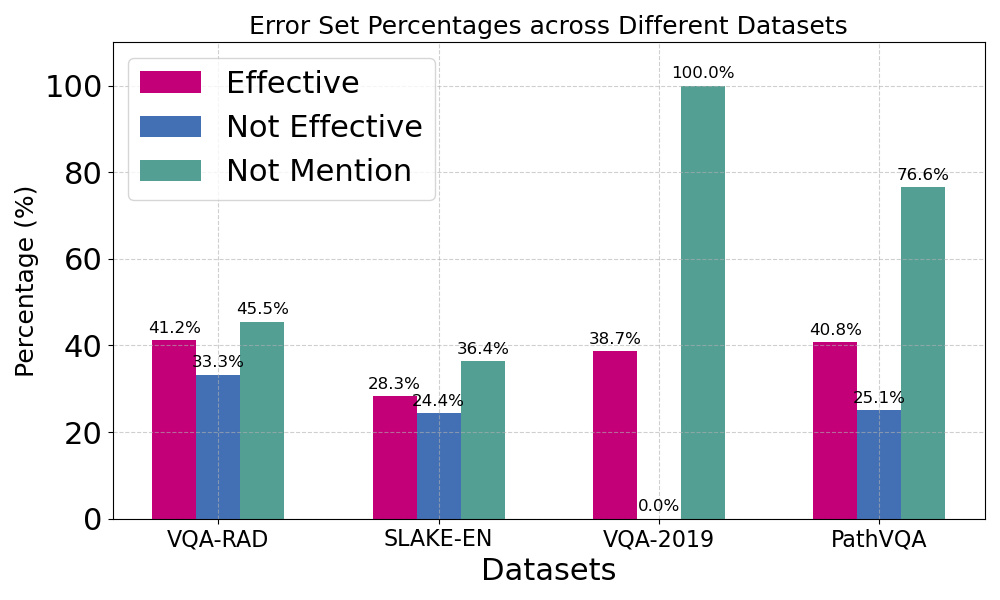
\includegraphics[width=0.45\textwidth]{image/Error_set.png}
% \caption{
% Error set percentages across different datasets: the proportion of the error set in zero-shot setting was classified based on the attitude of self-reflection 
% (The better the performance, the lower the bar).
% } 
% \vspace{-1em}
% \label{fig:Error set percentages}
% \end{figure}

% As seen in \autoref{fig:Error set percentages}, the "Not Effective" category has the lowest error proportion in four datasets. This indicates that when the model deems the rationale from the Initial Specialist insufficient to answer the question reasonably, modifications made during the reflection stage can prevent some errors, resulting in the lowest proportion in the error set. Therefore, this experiment demonstrates that Self-Reflection can enhance the model's ability to judge and solve problems in Follow-up Specialist, providing support for subsequent experiments and model improvements (An complete example in \autoref{fig:Case_study}).


% \section{Computing Resource Costs}
% \label{secH1}
% % MedCoT, while computationally more expensive than single-model methods, presents a trade-off that aligns with the complexities of real-world medical diagnostics. As demonstrated in the table below, MedCoT's hierarchical expert framework may require more processing time, but this is compensated by its ability to provide more accurate and interpretable diagnostic pathways. Such an approach better mirrors the multi-step decision-making process of medical professionals, where precision is paramount. 
% % A comparison of cost and latency across various baseline models—conducted on four NVIDIA GEFORCE RTX 3090 GPUs—reveals that, despite MedCoT’s higher computational overhead and latency relative to methods like Vanilla-CoT (which utilizes Gemini Pro for rationale querying) and MedThink, its performance gains are substantial. These improvements in accuracy and diagnostic reliability are especially critical in medical applications, where enhanced precision directly translates to improved patient outcomes. Thus, the additional computational cost is justified in light of the significant performance benefits MedCoT provides in medical contexts. \autoref{table:comparison} shows the experiment results.

% We compared the cost and latency of some baselines on 4 NVIDIA GEFORCE RTX 3090 GPUs, as shown in \autoref{table:comparison}. Although MedCoT incurs higher costs and latency compared to Vanilla-CoT (which derives answers by querying rationales using Gemini Pro) and MedThink, it exhibits a significant leap in performance. This performance improvement is particularly crucial in medical scenarios, enhancing reliability.

% \begin{table}[h!]
% \centering
% \caption{Cost, Latency, and VQA-RAD Accuracy for MedCoT, Vanilla (CoT), and MedThink.}
% \resizebox{\linewidth}{!}{
% \begin{tabular}{lccc}
% \toprule
% & \textbf{MedCoT (Ours)} & \textbf{Vanilla (CoT)} & \textbf{MedThink} \\ 
% \midrule
% \textbf{Cost (tokens/sample)} & 1550 & 1493 & - \\ 
% \textbf{Latency (seconds)} & 11.23 & 5.02 & 7.25 \\ 
% \textbf{VQA-RAD (accuracy)} & 87.50\% & 60.29\% & 83.50\% \\ 
% \bottomrule
% \end{tabular}
% }
% \label{table:comparison}
% \end{table}


% \section{Assessing the Impact of Different Prompts}
% \label{secH2}


% \begin{table*}[ht]
% \centering
% \caption{Prompt Modifications for Initial and Follow-up Specialists}
% \resizebox{\textwidth}{!}{
% \begin{tabular}{ccc}
% \toprule
% \textbf{Role} & \textbf{Type} & \textbf{Prompt} \\ 
% \midrule
% \textbf{Initial Specialist} & \textbf{Original} & As ... \textbf{experienced doctor}, next steps are required. Provide a reasonable rationale for the questions: \{question\} ... \\ 
% \textbf{Initial Specialist} & \textbf{Change} & Acting ... assistant to a \textbf{seasoned doctor}, ... explain why each question \{question\}... \\ 
% \textbf{Follow-up Specialist} & \textbf{Original} & ...Evaluate the effectiveness of the given rationale. \textbf{If effective}, summarize and refine it. If insufficient, ... \\ 
% \textbf{Follow-up Specialist} & \textbf{Change} & As an assistant to an experienced doctor, ... Check if the rationale: \{rationale\} is \textbf{useful}... \\ 
% \bottomrule
% \end{tabular}
% }
% \label{tab:Prompt}
% \end{table*}

% MedCoT, places significant emphasis on prompt engineering, which is inherently sensitive to minor variations in wording and structure. To assess the impact of these prompt variations on the generated rationales, we conducted an experiment where we modified the prompt wording and generated a new version of the rationale. The details of these prompt modifications are outlined in \autoref{tab:Prompt}.

% A comparison of the original and modified rationales was conducted by calculating their cosine similarity. The results indicated that the rationales remained semantically close, with an average similarity score exceeding 70\%. In the SLAKE-EN dataset, All the rationales had cosine similarity scores above 50\%, with an average of 74\%. Similarly, in the VQA-RAD dataset, 98.4\% of the rationales achieved similarity scores above 50\%, with an average score of 78.1\%. These findings demonstrate that changes in prompt wording did not lead to significant semantic divergence.

% To evaluate the practical implications of these modifications, we performed subsequent zero-shot experiments using both the original and modified rationales to query Gemini Pro. The resulting zero-shot scores were comparable across both versions, with performance differences constrained to within a 3\% margin. This consistency suggests that while variations in prompt wording can influence the generated rationales, their effect on model performance is relatively modest. 
% % The model exhibited robustness, as slight alterations in prompt structure did not lead to significant deviations in outcomes. These findings underscore the resilience of the model to prompt engineering variations, reinforcing its reliability for zero-shot tasks.
% The detailed results of this comparison are presented in \autoref{tab:Performance}.

% \begin{table}[h]
% \centering
% \caption{
% Performance Variations across Different Prompts.}
% \resizebox{\linewidth}{!}{
% \begin{tabular}{lccc}
% \toprule
% Dataset & Original Setting & Change Setting & Absolute Change \\
% \midrule
% VQA-RAD   & 60.29\%  & 57.45\%  & 2.84\%  \\
% SLAKE-EN  & 72.40\%  & 73.04\%  & 0.64\%  \\
% \bottomrule
% \end{tabular}
% }
% \label{tab:Performance}
% \end{table}






% \section{Prompt Template}
% \label{secG}
% \subsection{Initial Specialist CoT prompt}

% In this work, we introduce the templates for the Initial Specialist and the Follow-up Specialist Prompt for CoT, which utilize LLMs to generate rationales and optimize VQA pairs, thereby achieving hierarchical expert authentication. Furthermore, to enhance image information and mitigate potential loss of visual data, we employ LLMs to supplement image captions.

% \begin{tcolorbox}[colback=gray!20!white, colframe=gray!50!black, title=Initial Specialist CoT Prompt ($prompt_{\hat{i}}$)]
% As an agent/assistant of an experienced doctor, the next steps are required. \\
% - Provide a reasonable rationale for the questions: {question}  and image entered.\\
% - Please proceed with a step-by-step analysis and provide a rationale.


% \end{tcolorbox}
% \newpage

% \subsection{Follow-up Specialist Prompt}
% \label{followprompt}
% \begin{tcolorbox}[colback=gray!20!white, colframe=gray!50!black, title=Follow-up Specialist Self-Reflection Prompt ($prompt_{\hat{f}}$)]
% Please as an agent/assistant of an experienced doctor:
% Question and Image is also included, it is useful to provide the information\\
% - Existing Rationale: \{rationale\}; Task: Please judge whether this rationale is effectively valid for question and image. \\
% - If it is effective, summarize and refine the rationale to highlight key points, else the existing rationale is insufficient or irrelevant, generate a clear, more precise, and concise explanation.


% \end{tcolorbox}

% \subsection{Follow-up specialist Image Caption Prompt}
% \label{captionprompt}
% \begin{tcolorbox}[colback=gray!20!white, colframe=gray!50!black, title=Image Caption Prompt]
% Your task is to add a caption for the image, the example is \\
% - The image features a black and white X-ray of a person's chest, revealing their lungs and rib cage. ...[Few-shot Example of an Image]... Overall, the X-ray provides a comprehensive view of the person's respiratory system.\\ 
% - So this image caption can be:[caption]
% \end{tcolorbox}


% \begin{figure*}[t]
% \centering
% 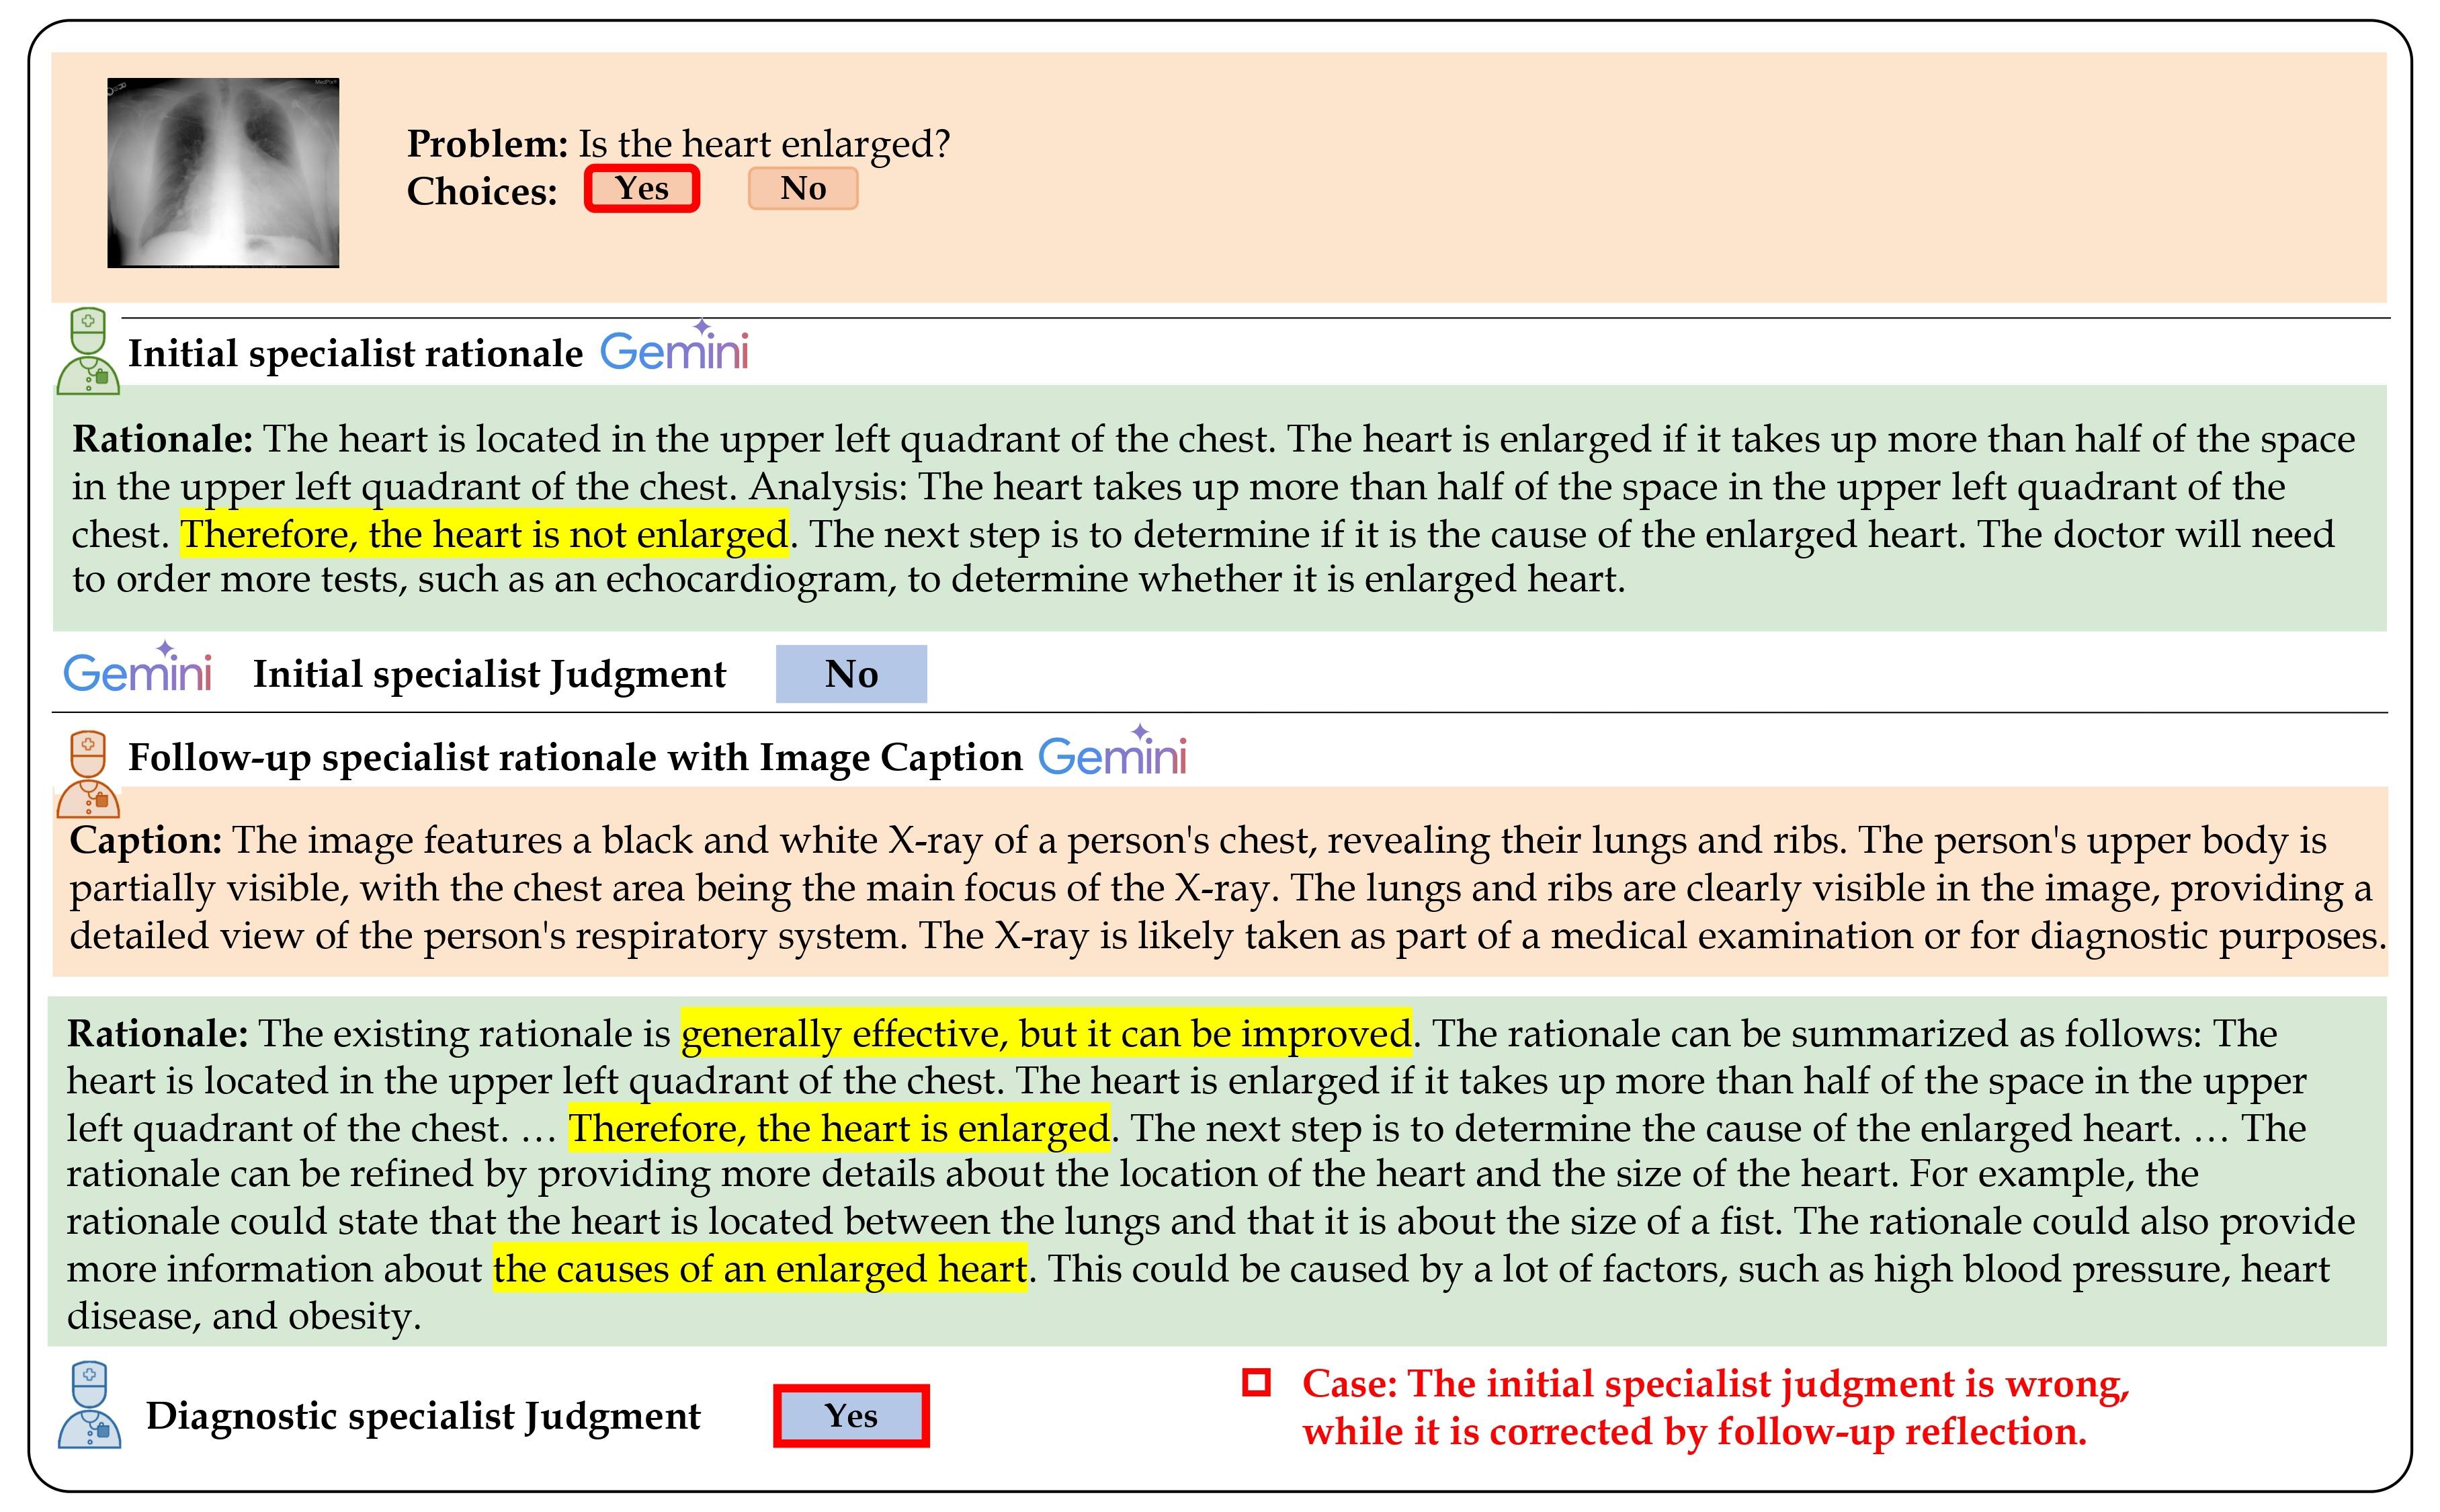
\includegraphics[width=\textwidth]{image/Case_study.jpg}
% \caption{
% Detailed Procedure of Specialist Self-Reflection and Diagnostic Correction: 
% It starts with the initial problem statement, followed by the Initial Specialist's rationale and judgment.
% % The process of self-reflection and correction in a specialist's diagnostic judgment. 
% The Follow-up Specialist provides a detailed image caption and refines the rationale by Self-Reflection. 
% The final diagnostic judgment confirms the corrected assessment, demonstrating the importance of self-reflection for accurate medical diagnoses.
% } 
% \label{fig:Case_study}
% \end{figure*}



\end{document}



